\documentclass[12pt,tightenlines,letterpaper]{scrartcl}
\usepackage{lmodern}
\usepackage{ifxetex,ifluatex}
\usepackage{fixltx2e} % provides \textsubscript
\ifnum 0\ifxetex 1\fi\ifluatex 1\fi=0 % if pdftex
  \usepackage[T1]{fontenc}
  \usepackage[utf8]{inputenc}
\else % if luatex or xelatex
  \ifxetex
    \usepackage{mathspec}
  \else
    \usepackage{fontspec}
  \fi
  \defaultfontfeatures{Ligatures=TeX,Scale=MatchLowercase}
\fi

%%% Needed to write listtodonotes, and listofalgorithms, but the problem is listoftodonotes
% \usepackage{morewrites}
\usepackage[
HomeHTMLFilename=index,     % Filename of the homepage.
%HTMLFilename={node-},       % Filename prefix of other pages.
%IndexLanguage=english,      % Language for xindy index, glossary.
latexmk,                    % Use latexmk to compile.
%   OSWindows,                  % Force Windows. (Usually automatic.)
mathjax,                    % Use MathJax to display math.
]{lwarp}


\title{Block Chain Notes}
\author{David Li}
\setcounter{tocdepth}{2} % Include subsections in the \TOC.
\setcounter{secnumdepth}{2} % Number down to subsections.
\setcounter{FileDepth}{0} % Split \HTML\ files at sections, in this case chapters?, 0 for chapters?
\booltrue{CombineHigherDepths} % Combine parts/chapters/sections
\setcounter{SideTOCDepth}{1} % Include subsections in the side\TOC
\HTMLAuthor{David Li} % Sets the HTML meta author tag.
\HTMLLanguage{en-US} % Sets the HTML meta language.
\HTMLDescription{A list of cheatsheets for courses at the University of Victoria}% Sets the HTML meta description.
\HTMLFirstPageTop{ CheatSheets \fbox{
\includegraphics[width=1\linewidth]{Images/Ethereum-Cover.png}}}
\HTMLPageTop{\fbox{
\includegraphics[width=1\linewidth]{Images/Ethereum-Cover.png}}}
\HTMLPageBottom{Made by David Li}
\newcommand{\printTitle}{Insert a title Here} 
\usepackage{graphicx} % Required for including pictures
\graphicspath{{Images/}} % Specifies the directory where pictures are stored

%%%% Useful Packages loaded without much configuration %%%%%%
\usepackage[margin=2.54 cm]{geometry} % Set dimensions for page layout
\usepackage{kpfonts}	    % Fonts used in the title page
\usepackage{eso-pic}        % Background pictures in the title page
\usepackage{tcolorbox}		% Fancy Math equations	
\usepackage{tabularx}		% Tabulars with adjustable-width columns
\tcbuselibrary{skins} 	% used with tcolorbox 
\usepackage{transparent}	% Create transparent background images
\usepackage{lipsum}  % Garbage text
\usepackage{url}	 % links to websites
\usepackage{pdfpages} % to include pdf pages
\usepackage{booktabs}	% Make high quality tables
\usepackage{colortbl}	% Color tables
\usepackage{xfrac}		% Make fractions nice in tables
\usepackage{enumitem}	% itemize, enumerate
\usepackage{array}
\usepackage{setspace}   % double spacing as required in UVIC co-op reports
\usepackage{titlesec} % Select alternative section titles
\titlespacing*{\section}
{0pt}{5.5ex plus 1ex minus .2ex}{4.3ex plus .2ex}	% Not sure about this spacing
\usepackage{multirow} % Create tabular cells spanning multiple rows.

\usepackage{float}    % used for float­ing ob­jects such as fig­ures and ta­bles.
\usepackage{caption}
%\captionsetup[figure]{labelfont=sf,textfont={sf}}
%\captionsetup[table]{labelfont=sf,textfont={sf}}
% \usepackage{parskip} % no indents, don't use in lwarp
\usepackage{tikz}	 % for drawings and cool graphics

%% Math packages %%
\usepackage{siunitx}	% SI units
\usepackage{mathtools}	% LOAD MATH
\usepackage{amssymb}  	% MATH Symbols


%%%%%%%%%% COLORS %%%%%%%%%%%%%%%%%%%%%%%%%%%%%
\definecolor{titlepagecolor}{cmyk}{1,.60,0,.40}

%%%%%%%%%%%%%%%%%%%%%%%%%%%%%%%%%%%%%%%%%%%%%%%%%%%%%%%%%%%%%%%%%%%%%%
%%%%%%%%%%%%%%%%%%%%%%%%%%%% CODE STYLINGS %%%%%%%%%%%%%%%%%
%%%%%%%%%%%%%%%%%%%%%%%%%%%%%%%%%%%%%%%%%%%%%%%%%%%%%%%%%%%%%%%%%%%%%%%%

\usepackage{listings} % For source code
\DeclareCaptionFont{white}{\color{white}}
\DeclareCaptionFormat{listing}{\colorbox{titlepagecolor}{\parbox{1\textwidth}{#1#2 \quad #3}}}
\captionsetup[lstlisting]{format=listing,labelfont=white,textfont={white,sf}} % for fancy boxes

\lstdefinestyle{default}{frame=tb,
	aboveskip=3mm,
	backgroundcolor=\color{cornsilk},
	belowskip=3mm,
	showstringspaces=false,
	columns=flexible,
	basicstyle={\ttfamily},
	numbers=none,
	numberstyle=\tiny\color{red},
	keywordstyle=\color{blue},
	commentstyle=\color{green},
	stringstyle=\color{purple},
	morekeywords={fclose, exit, printf, fscanf, strcpy, strlen,
		strcmp, fprintf},
	breaklines=true,
	breakatwhitespace=true,
	tabsize=3,
	captionpos=t,
	columns=flexible,
}
%%%%%%%%%%%%%%%%%%%%%%%%%%%%%%%
%%%%%% SQL style setup %%%%%%%%
\makeatletter
\newcommand{\lstuppercase}{\uppercase\expandafter{\expandafter\lst@token
		\expandafter{\the\lst@token}}}	%%%UPPERCASE SQL%%%%
\newcommand{\lstlowercase}{\lowercase\expandafter{\expandafter\lst@token
		\expandafter{\the\lst@token}}} %%% REGULAR CASE %%%%
\makeatother

\definecolor{mauve}{rgb}{0.58,0,0.82}
\lstdefinestyle{Oracle}{basicstyle=\ttfamily,
	keywordstyle=\lstuppercase,
	backgroundcolor=\color{cornsilk},
	emphstyle=\itshape,
	showstringspaces=false,
	morekeywords={ACCESS, MOD, NLS_DATE_FORMAT, NVL, REPLACE, SYSDATE,
		TO_CHAR, TO_NUMBER, TRUNC},
	numberstyle=\tiny\color{black},
	keywordstyle=\color{red},
	commentstyle=\color{green},
	stringstyle=\color{mauve},
	columns=flexible,
}
%%%%%%%%%%%%%%%%%%%%%%%%%%%%%%%%%%%%%%%%%%%%%%%%
%%%%%%%%%%%%%%%%%%%%%JAVA %%%%%%%%%%%%%%%%%%%%%%
\definecolor{javared}{rgb}{0.6,0,0} % for strings
\definecolor{javagreen}{rgb}{0.25,0.5,0.35} % comments
\definecolor{javapurple}{rgb}{0.5,0,0.35} % keywords
\definecolor{javadocblue}{rgb}{0.25,0.35,0.75} % javadoc
\lstdefinestyle{myJava}{frame=tb,
	basicstyle=\ttfamily,
	backgroundcolor=\color{cornsilk},
	keywordstyle=\color{javapurple}\bfseries,
	stringstyle=\color{javared},
	commentstyle=\color{javagreen},
	morecomment=[s][\color{javadocblue}]{/**}{*/},	% Make comments blue
	morecomment=[is]{/*}{*/},  % Remove comments
	stepnumber=2,
	numbers=left,    % print line numbers
	numbersep=10pt,
	tabsize=4,
	showspaces=false,
	showstringspaces=false,
	linewidth=\textwidth,
	columns=flexible,			% Important for keeping text in the frame
	breaklines=true,
}

%%%%%%%%%%%%%%%%%% ENDJAVA %%%%%%%%%%%%%%%%%%%%%
%%%%%%%%%%%%%%%%%%%%%%%%%%%%%%%%%%%%%%%%%%%%%%%%

%%%%%%%%%%%%%%%%%%%%%%%%%%%%%%%%%%%%%%%%%%%%%%%%%%
%%%%%%%%%%%%%%%%%%%%% JAVASCRIPT%%%%%%%%%%%%%%%%%%%
\lstdefinelanguage{JavaScript}{frame=tb,
	keywords={typeof, new, true, false, catch, function, return, null, catch, switch, var, if, in, while, do, else, case, break},
	keywordstyle=\color{blue}\bfseries,
	ndkeywords={class, export, boolean, throw, implements, import, this},
	ndkeywordstyle=\color{darkgray}\bfseries,
	identifierstyle=\color{black},
	sensitive=false,
	comment=[l]{//},
	morecomment=[s]{/*}{*/},
	commentstyle=\color{purple}\ttfamily,
	stringstyle=\color{red}\ttfamily,
	morestring=[b]',
	morestring=[b]"
}
\definecolor{cornsilk}{rgb}{1.0, 0.97, 0.86}
\lstdefinestyle{myJavaScript}{
	language=JavaScript,
	backgroundcolor=\color{cornsilk},
	extendedchars=true,
	basicstyle=\ttfamily,
	showstringspaces=false,
	showspaces=false,
	tabsize=2,
	breaklines=true,
	showtabs=false,
	captionpos=t,
}
%%%%%%%%%%%%%%%%%%%%%%%%%%%%%%%%%%%%%%%%%%%%%%%%%%
%%%%%%%%%%%%%% END CODE STYLINGS %%%%%%%%%%%%%%%%%
%%%%%%%%%%%%%%%%%%%%%%%%%%%%%%%%%%%%%%%%%%%%%%%%%

%%%%%%%%%%%%%%%%%%%%%%%%%%%%%%%%%%%%%%%%%%%%%%%%%%%%%%%%%%%%
%%%%%%%%%%%%%%%%%%%%%%%%% FORMATTING %%%%%%%%%%%%%%%%%%%%%%%
% Format TOC, header, footers and chapters
%% tocloft settings
\usepackage[titles]{tocloft}	% Pro­vides con­trol over the ty­pog­ra­phy of the Ta­ble of Con­tents, List of Fig­ures and List of Tables
\setlength{\cftbeforesecskip}{3pt}
% End tocloft settings

\usepackage{sectsty} % used to color chapter and sections
%\renewcommand{\cftpartleader}{\cftdotfill{\cftdotsep}} % for parts
%\renewcommand{\cftchapleader}{\cftdotfill{\cftdotsep}} % for chapters
\renewcommand{\cftsecleader}{\cftdotfill{\cftdotsep}} % for sections, if you really want! (It is default in report and book class (So you may not need it).
% ----------------------------------------------------------------
%\renewcommand{\cftdotsep}{0}	 % dots in the title page
% \renewcommand{\cftsectleader}{\bfseries\cftdotfill{\cftsecdotsep}}% dot leaders in bold 


   % NUMBERING IN TOC FOR SUMMARY SECTION %%%%%%%%
   \newcommand{\mysection}[2]{
   	\setcounter{section}{#1}
   	\setcounter{subsection}{0}
   	\section*{#2}
   	\addcontentsline{toc}{section}{#2}
   }
  
   %%%%%%%%%%%%%%%%%%%%%%%%%%%%%%%%
    %CHAPTER Title formatting
	\definecolor{myText}{HTML}{2B2B2B}
	\definecolor{myChap}{HTML}{000066}
	\definecolor{mySect}{HTML}{336699}
	\definecolor{mySubSect}{HTML}{2088B2}

    \renewcommand{\sectionmark}[1]{\markboth{\thesection.\ #1}{}}
    
    % SET UP COLOURS FOR HEADINGS IN THE REPORT
    \sectionfont{\color{mySect}}  % sets colour of sections
    \subsectionfont{\color{mySubSect}}  % sets colour of subsections
    \subsubsectionfont{\color{mySubSect}}  % sets colour of subsubsections
    \subparagraphfont{\color{red}}		    % sets colour of paragraphs

   	%%%%%%%%%%%%%%%%%%%%%%%%%%%%%%%%%%%%%%%%%%%%%%%%%%%%%%%%%%%%%%%%
   	%CHANGE  GLOBAL TEXT COLOR %%%%%%%%%%%%%%%%%%%%%
   	\makeatletter
   	\newcommand{\globalcolor}[1]{%
   		\color{#1}\global\let\default@color\current@color
   	}
   	\makeatother
   	
   	% Edit the global text colour, make the report easier to read for digital screens or print.
   	%\AtBeginDocument{\globalcolor{myText}}
   	
   %%%%%%%%%%%%%%%%%%%%%%%%%%%%%%%%%%%%%%%%%%%%%%%%%%%%%%%
   % SET UP COMBINED LOT and LOF 	%%%%%%%
   %	CONFIG LOL					%%%%%%%
   %%%%%%%%%%%%%%%%%%%%%%%%%%%%%%%%%%%%%%%%%%%%%%%%%%%%%%%%%%%
%   \makeatletter
%   \def\ext@figure{lot}
%   \makeatother\

%	\setcounter{tocdepth}{4} % INCLUDE SUBSUBSECTIONS IN TOC
  % \renewcommand{\lstlistingname}{Listing}	% Change caption in code listing
   %\renewcommand{\lstlistlistingname}{List of Scripts}     % CHANGE THE HEADER IN TOC
   
   % Create List of Figures and Tables in LATEX
%   \renewcommand*\listtablename{List of Figures and Tables}
%   \renewcommand{\cftfigpresnum}{Figure~}
%   \renewcommand{\cftfigaftersnum}{:}
%   \setlength{\cftfignumwidth}{5.5em}
%   \renewcommand{\cfttabpresnum}{Table~}		
%   \renewcommand{\cfttabaftersnum}{:}
%   \setlength{\cfttabnumwidth}{5.5em}
   
%   %CONFIG SCRIPTS in TOC %%%%%%
%   \makeatletter
%   \AtBeginDocument{%	Add the word Program in front of the caption in TOC and listing
%   	\renewcommand\lstlistoflistings{\bgroup
%   		\let\contentsname\lstlistlistingname
%	\def\l@lstlisting##1##2{\@dottedtocline{1}{1.3em}{3em}{\bfseries Script 
%				##1}{##2}}
%   		\let\lst@temp\@starttoc \def\@starttoc##1{\lst@temp{lol}}%
%   		\tableofcontents \egroup}
%   }
%   \makeatother
%   
%   %MAKE SPACING THE SAME AS IN THE LOT AND LOF in Programs %%%%%%
%%   \makeatletter
%%   \let\my@chapter\@chapter
%%   \renewcommand*{\@chapter}{%
%%   	\addtocontents{lol}{\protect\addvspace{10pt}}%
%%   	\my@chapter}
%%   \makeatother
   
%%%%%%%%%%%%%%%%%%%%%%%%%%%%%%%%%%%%%%%%%%%%%%%%%%%%%%%%%%%%%%%%%%
%%%%%% SET UP BIBLIOGRAPHY  %%%%%%%%%%%%%%%%%%%%%%%%%%%%%%%%%%%%%%%%%%%
%%%%%%%%%%%%%%%%%%%%%%%%%%%%%%%%%%%%%%%%%%%%%%%%%%%%%%%%%%%%%%%%%%
% See https://tex.stackexchange.com/questions/6967/how-to-split-bibliography-into-works-cited-and-works-not-cited?noredirect=1&lq=1
% https://tex.stackexchange.com/questions/128959/multiple-bibiographies-using-biblatex-and-resetting-numbers
\usepackage[defernumbers=true,backend=bibtex,sorting=none]{biblatex}	% Sort by citation order
\DeclareBibliographyCategory{cited}
\AtEveryCitekey{\addtocategory{cited}{\thefield{entrykey}}}
\defbibheading{bibliography}[\bibname]{%
  	\subsubsection*{#1}}%	% set up bibliography as a section 
  	%\markboth{\thesection.\ #1}{}}	%label at upper right corner in header

\usepackage[titletoc]{appendix}	%% appendix will be in the toc
% What I want is References and subsections or paragraphs 

% This created 5. Cited References and 6. General References
%\usepackage[nottoc,numbib]{tocbibind}	% Label the Biblography in the TOC
%\defbibheading{bibliography}[\bibname]{%
%  	\section{#1}%	% set up bibliography as a section 
%  	\markboth{\thesection.\ #1}{}}	%label at upper right corner in header
\newcommand{\onlineCite}{[Online] Available: }	% Used in BIBLIOGRAPHY
% Load all references 
\nocite{*}

%%%%%%%%%%%%%%%%%%%%%%%%%%%%%%%%%%%%%%%%%%%%%%%%%%%%%%%%%%%%%%%%%%%
%%%%%%%%% CUSTOMIZE GLOSSARY %%%%%%%%%%%%%%%%%%%%%%%%
\usepackage[toc,nopostdot,xindy]{glossaries} % included in toc and keep track of technical words and definition and remove dots at the end

% glossary definitions as bold
%\defglsentryfmt{\color{black}\bfseries\glsgenentryfmt}

% custom glossary style that contains the pages that contains the glossary terms, and bolded glossary entries.
%\newglossarystyle{myGloss}{%
%	\setglossarystyle{list}
%	\renewcommand*{\glossentry}[2]{%
%		\item[\textbf{\glsentryitem{##1}}%
%		\textbf{\glstarget{##1}}{\textbf{\glossentryname{##1}:}}]
%		\glossentrydesc{##1}\glspostdescription\space See p.\space ##2} 
%}
%\setglossarystyle{listhypergroup}
%\setglossarystyle{myGloss}

% Set up roman numercals page numbering for front matter, letter of transmittal, and table of contents.
% Commentout for lwarp
\newcommand\frontmatterNumbering{%
	\cleardoublepage
	%\@mainmatterfalse
	\pagenumbering{roman}}
\renewcommand{\familydefault}{\sfdefault} % Nice font formatting

\let\cleardoublepage\clearpage % prevent book from create extra pages bewteen chapters

%%% Set up verbatim for WYSIWYG formatting for letter
\usepackage[T1]{fontenc}%  selects EC fonts
\usepackage{verbatim}%     configurable verbatim
\makeatletter
\def\verbatim@font{\normalfont% select the font
	\let\do\do@noligs
	\verbatim@nolig@list}
\makeatother



%%%% Set up headers %%%%
\usepackage{fancyhdr}	% Controls headers and footers
   \fancypagestyle{plain}{
   	\fancyhf{}
   	\setlength{\headheight}{15pt} 
   	\fancyhead[L]{ \textsf{Creating transparent and efficient transactions through smart contracts and blockchain}}
   	%\fancyhead[R]{\textsf{\leftmark}}
   	\fancyfoot[C]{\textsf{ENGR 446: Technical Report}}
   	\fancyfoot[L]{\textsf{David Li}}
   	\fancyfoot[R]{\textsf{\thepage}}
   	\renewcommand{\headrulewidth}{0.4pt}
   	\renewcommand{\footrulewidth}{0.4pt}
   }
   
    % NUMBERING IN TOC FOR SUMMARY SECTION %%%%%%%%
      \newcommand{\mychapter}[2]{
      	\setcounter{chapter}{#1}
      	\setcounter{section}{0}
      	\chapter*{#2}
      	\addcontentsline{toc}{chapter}{#2}
      }
     
      %%%%%%%%%%%%%%%%%%%%%%%%%%%%%%%%
      % Remove Footer on select pages
      \fancypagestyle{nofooter}{%
      	\fancyfoot{}%
      	\fancyhead{}%
      }

% Diagram, adjust big picture
\usepackage{adjustbox}

%\usepackage[x11names,table]{xcolor}
%\DeclareCaptionFont{blue}{\color{LightSteelBlue3}}

\newcommand{\foo}{\color{blue}\makebox[0pt]{\textbullet}\hskip-0.5pt\vrule width 1pt\hspace{\labelsep}}



%%% Following lwarps documentation hyperref will be loaded last
%CHANGE Link colours as needed
\definecolor{linkColor}{HTML}{453737}	

\usepackage{hyperref}	% Create links in document
\hypersetup{linktocpage}	% Allow clickable links
\hypersetup{
    bookmarks=true,         % show bookmarks bar?
    unicode=false,          % non-Latin characters in Acrobat’s bookmarks
    pdftoolbar=true,        % show Acrobat’s toolbar?
    pdfmenubar=true,        % show Acrobat’s menu?
    pdffitwindow=false,     % window fit to page when opened
    pdfstartview={FitH},    % fits the width of the page to the window
    pdftitle={ENGR 446: Smart Contracts},    % title
    pdfauthor={David Li},     % author	
    %linktoc=all,     %set to all if you want both sections and subsections linked
	colorlinks   = true, %Colours links instead of ugly boxes
	urlcolor     = blue, %Colour for external hyperlinks
	linkcolor    = blue, %Colour of internal links
	citecolor   = black %Colour of citations
}
%%%%%%%%%%%%%%%%%%%%%%%%%%%%%%%%%%%%%%%%%%%%%%%%%%
%%%%%%%%%%% END PREAMBLE %%%%%%%%%%%%%%%%%%%%%%%%%
%%%%%%%%%%%%%%%%%%%%%%%%%%%%%%%%%%%%%%%%%%%%%%%%%%
\newcolumntype{Y}{>{\raggedleft\arraybackslash}X}

\definecolor{otherColour}{HTML}{F7ADBC}
\definecolor{mainnet}{HTML}{29B6AF}
\definecolor{kovan}{HTML}{7057ff}
\definecolor{ropsten}{HTML}{FF4A8D}
\definecolor{rinkeby}{HTML}{F6C343}

\tcbset{tab1/.style={fonttitle=\bfseries\large,fontupper=\normalsize\sffamily,
		colback=yellow!10!white,colframe=ropsten!75!black,colbacktitle=rinkeby!40!kovan,
		coltitle=black,center title,freelance,frame code={
			\foreach \n in {north east,north west,south east,south west}
			{\path [fill=red!75!black] (interior.\n) circle (3mm); };},}}

\tcbset{tab2/.style={enhanced,fonttitle=\bfseries,fontupper=\normalsize\sffamily,
		colback=rinkeby!5,colframe=kovan,colbacktitle=ropsten!10,
		coltitle=mainnet!5!black,center title}}
		
%%%%%%%%%%%%%%%%%%%%%%%%%%%%%%%%%%%%%
%%%%%%%%%% BEGIN GLOSSARIES %%%%%%%%%%%%%%%
%%%%%%%%%%%%%%%%%%%%%%%%%%%%%%%%%%%%%%%%%%%

\newglossaryentry{sql}
{
	name={SQL},
	description={SQL (Structured Query Language) is a standard interactive and programming language for getting information from and updating a database.},
	first={Structured Query Language (SQL)},
	long={Structured Query Language}
}
\newglossaryentry{sd}
{
	name={System Documentation},
	text={documentation},
	description={A collection of documents that describes the requirements, \newline capabilities, limitations, design, operation, and maintenance of a system, such as a communications, computing, or information processing system.},
	long={System Documentation}
}

\newglossaryentry{sharepoint}
{
	name={SharePoint},
	description={A browser-based collaboration and document management platform from Microsoft. },
	first={Microsoft SharePoint},
	long={Microsoft Lync}
}
\newglossaryentry{JIRA}
{
	name={JIRA},
	description={Software development tool  that is mainly used for bug tracking and project management by \gls{agile} teams. },
}
\newglossaryentry{agile}
{
	name={agile},
	description={Iterative approach to software delivery that creates software incrementally from the beginning of the project, instead of trying to deliver it all at once near the end.},
}
\newglossaryentry{scrum}
{
	name={Scrum},
	description={Scrum is an iterative and incremental agile software development framework for managing product development.}
}
\newglossaryentry{kanban}
{
	name={Kanban},
	description={Kanban is a method for managing knowledge work which balances the demand for work to be done with the available capacity to start new work.}
}
\newglossaryentry{Confluence}
{
	name={Confluence},
	description={Team collaboration software which allows team members to create, share and collaborate information.},
}

\newglossaryentry{jql}
{
	name={JQL},
	description={Structured queries to search for issues in JIRA. It is the most flexible way to search for issues in JIRA and similar to \gls{sql} },
	first={JIRA Query Language (JQL)},
	long={JIRA Query Language}
}
\newglossaryentry{excel}
{
	name={Excel},
	description={Electronic Spreadsheet Program that is used for storing, organizing and manipulating data.},
	first={Microsoft Excel},
	long={JIRA Query Language}
}
\newglossaryentry{MOTI}
{
	name={MOTI},
	description={Previous Employeer},
	first={INSERT PREVIOUS EMPLOYEER},
	long={Previous Employeer}
}
\newglossaryentry{IMB}
{
	name={IMB},
	description={Infomration DIVIOSN},
	long={Infomration DIVIOSN},
	first={IInfomration DIVIOSN}
}
\newglossaryentry{wiki}
{
	name={wiki},
	description={a website that allows collaborative editing of its content and structure by its users.}
}
\newglossaryentry{ssot}
{
	name={single source of truth},
	description={one source of data that everyone in a organization agrees is the real, trusted number for some operating data.}
}
\newglossaryentry{issue}
{
	name={issue},
	description={unit of work to accomplish an improvement in a system such as access requests and tasks.}
}

\newglossaryentry{Bitcoin}
{
	name={Bitcoin},
	description ={
		a type of digital currency in which encryption techniques are used to regulate the generation of units of currency and verify the transfer of funds, operating independently of a central bank
	}
}
%%% Add in Solidity is a programming language specified designed for smart contracts. It takes inspiration from javascript, python and C++. 
\newglossaryentry{blockchain}
{
	name={blockchain},
	description ={
		A blockchain is a digitized, decentralized, public ledger of all cryptocurrency transactions.  It constantly grows as the most recent transactions (blocks) are appended in chronlogical order.
		%Constantly growing as \textit{completed} blocks (the most recent transactions) are recorded and added to it in chronological order, it allows market participants to keep track of digital currency transactions without central recordkeeping.
	}
}


\newglossaryentry{DApp}
{
	name={Dapp},
	description ={
		Decentralized Application have backend code running on a decentralized peer-to-peer network and not controlled by a single entity. In a decentralized application transactions are versified through consensus of multiple users.
	},
	first={Decentralized Application(DApp)}
}

% cryptocurrency gls
\newglossaryentry{Ethereum}
{
	name={Ethereum},
	description={
		an open software platform based on blockchain technology that enables developers to build and deploy decentralized applications. The main unit of currency is ether.
	}
}

\newglossaryentry{HyperLedger}
{
	name={HyperLedger},
	description ={
		group of open-source blockchain technologies started by the Linux Foundation
	}
}

\newglossaryentry{HyperLedger Composer}
{
	name={HyperLedger Composer},
	description ={
		permissioned blockchain that defines assets, business rules, and participants, and access controls for existing roles and types of transactions.
	}
}

\newglossaryentry{MetaMask}
{
	name={MetaMask},
	description ={
		is a browser plugin that allows users to make Ethereum transactions through regular websites
	}
}



\newglossaryentry{smart contract}
{
	name={smart contract},
	description ={
		computer program that directly controls transfer of digital currencies or assets under predefined conditions and used to automatic transactions on the blockchain. These transactions are trackable and irreservable.
	}
}

\newglossaryentry{side chains}
{
	name={side chains},
	description= {
	are emerging mechanisms enable secure transfer of digital assets and tokens between blockchains. Attached to the parent blockchain using a two-way peg, sidechains are a separate blockchain and enables interchangeability of assets at a predetermined rate \cite{sideChains:Online}. 
	}
}
%% Software Tools
\newglossaryentry{git}
{
	name={git},
	description ={
			the most popular version control system used for tracking changes in source code and coordinating work on those files among multiple people.
	}
}


\newglossaryentry{GitLab}
{
	name={GitLab},
	description ={
		GitLab is an online Git repository manager with a wiki, issue tracking, and used to manage \gls{git} repositories on a centralized server
	}
}

\newglossaryentry{SHA-256}
{
	name={SHA-256},
	description ={
		cryptographic hash function that takes an input of a random size and produces an output of a fixed size. Hash functions are powerful because they are \textit{one-way}. What this is means is, it is possible for anyone to use a hash function to produce an output when given an input. However, it is impossible to use the output of the hash function to reconstruct its given input.
	},
	first={Secure Hash Algorithm-256}
}


\newglossaryentry{NFT}
{
	name={NFT},
	description ={
		is a special type of cryptographic token which represents something unique; non-fungible tokens are thus not interchangeable. This is different than most tokens such as ERC20. Used to represent unique assets, such as houses and cryptokitties.
	},
	first={Non-fungible token (NFT)}
}
%%%%%%%%%%%%%%%%%%%%%%%%%%%%%%%%%%%%
%%%%%%%%% END GLOSSARIES %%%%%%%%%%%%%%%
%%%%%%%%%%%%%%%%%%%%%%%%%%%%%%%%%%%%%%%
\makeglossaries
%%%%%%%%%%%%%%%%%%%%%%%%%%%%%%%%%%%%%%%%%%%%%%%%%%%%%%%%%%%%%%%%%%%
%%%%	Command to ensure  glossary can be properly printed %%%%%%%%%%
%%%% makeindex -l -s document.ist -o document.gls document.glo %%%%%%%%%
%%%%	Use name of latex document								%%%%%%%%%%%
%%%%%%%%%%%%%%%%%%%%%%%%%%%%%%%%%%%%%%%%%%%%%%%%%%%%%%%%%%%%%%%%%%%%%%%%%%%
%%%% OR use makeglossaries %%%%%%%%%%%%%%%%%%%%%%%%%%%%%%%%%%%%%%%%%%%%%%%%
%%%%%%%%%%%%%%%%%%%%%%%%%%%%%%%%%%%%%%%%%%%%%%%%%%%%%%%%%%%%%%%%%%%%%%
% Add Gas limit and gas, explain that gas limit is varies depending on what the miners decide on. Reference the crazy fluencance in ropsten testnet.
\makeglossaries
%\newcommand{\onlineCite}{[Online] Available}
\begin{filecontents*}{ENGR003.bib}
@Misc{sharepoint:Online,
	howpublished = { \onlineCite \url{https://support.office.com/en-us/article/What-is-SharePoint-97b915e6-651b-43b2-827d-fb25777f446f}},
	title = {What is SharePoint? - Office Support},
	note = {Accessed December 11, 2016},
}
@Misc{issueDefinition:Online,
	howpublished = { \onlineCite \url{https://confluence.atlassian.com/jira064/what-is-an-issue-720416138.html}},
	title = {What is an Issue},
	note = {Accessed December 11, 2016},
}

@Misc{PermissionsOverview:Online,
	howpublished = { \onlineCite \url{https://confluence.atlassian.com/jirasoftwarecloud/permissions-overview-764478244.html}},
	title = {Permissions overview },
	note = {Accessed December 13, 2016},
}
@Misc{NASA:Online,
	howpublished = { \onlineCite \url{http://summit.atlassian.com/archives/2010/presentations/collaboration-and-projects/confluence-wiki-at-nasa.jsp}},
	title = {Confluence at NASA: Where No Wiki Has Gone Before },
	note = {Accessed December 13, 2016},
}
@Misc{issues:Online,
	howpublished = { \onlineCite \url{https://confluence.atlassian.com/jirakb/crashes-and-performance-issues-troubleshooting-203394749.html}},
	title = {Crashes and Performance Issues Troubleshooting},
	note = {Accessed December 15, 2016},
}
@Misc{JAC:Online,
	howpublished = { \onlineCite \url{https://confluence.atlassian.com/doc/integrating-jira-and-confluence-2825.html}},
	title = {Integrating JIRA and Confluence},
	note = {Accessed December 17, 2016},
}
@Misc{confluence:Online,
	howpublished = { \onlineCite \url{https://confluence.atlassian.com/doc/integrating-jira-and-confluence-2825.html}},
	title = {Advanced and Special Uses of Confluence},
	note = {Accessed December 17, 2016},
}

@misc{bitcoinWhitePaper:Online,
	howpublished = { \onlineCite \url{https://bitcoin.org/bitcoin.pdf}},
	title = {Bitcoin White Paper},
	note = {Accessed April 25, 2018},
}

@misc{bitCoinProblems:Online,
	howpublished = { \onlineCite \url{https://www.forbes.com/sites/forbestechcouncil/2018/03/29/the-problems-with-bitcoin-and-the-future-of-blockchain}},
	author = {Saeed Elnaj},
	title = {The Problems With Bitcoin And The Future Of Blockchain
	},
	note = {Accessed May 06, 2018},
}
@misc{ethereumWhitePaper:Online,
	howpublished = { \onlineCite \url{https://github.com/ethereum/wiki/wiki/White-Paper}},
	title = {Ethereum White Paper},
	note = {Accessed April 25, 2018},
}

@misc{hyperledgerComposer:Online,
	howpublished = { \onlineCite \url{https://www.hyperledger.org/wp-content/uploads/2017/05/Hyperledger-Composer-Overview.pdf}},
	title = {Hyperledger Composer Overview},
	note = {Accessed May 27, 2018},
} 


// Finish off smart Contracts session with this reference
@misc{funnyJoke:Online,
	title = {Yes, this kid really just deleted 300 MILLION by messing around with Ethereum’s smart contracts.},
	author = {Thijs Maas},
	howpublished = {\onlineCite \url{https://hackernoon.com/yes-this-kid-really-just-deleted-150-million-dollar-by-messing-around-with-ethereums-smart-2d6bb6750bb9}},
	note = {Accessed May 29, 2018},
}

@Article{Sillaber2017,
author="Sillaber, Christian
and Waltl, Bernhard",
title="Life Cycle of Smart Contracts in Blockchain Ecosystems",
journal="Datenschutz und Datensicherheit - DuD",
year="2017",
month="Aug",
day="01",
volume="41",
number="8",
pages="497--500",
abstract="This paper discusses the life cycle of decentralized smart contracts, i.e. digital and executable representations of rights and obligations in a multi-party environment. The life cycle relies on blockchain technology, i.e. a distributed digital ledger, to ensure proper implementation and integrity of the smart contracts. The life cycle consists of four subsequent phases: Creation, freezing, execution, and finalization. For each phase actors and technological services are identified and explained in detail. With the life cycle at hand, risks and limitations of smart contracts and the underlying blockchain technology are briefly discussed.",
issn="1862-2607",
doi="10.1007/s11623-017-0819-7",
url="https://doi.org/10.1007/s11623-017-0819-7"
}

@misc{cryptozombies,
 author = {Loom Network},
 title = {Cryptozombies Solidity Tutorial},
 url = {https://cryptozombies.io/},
 lastchecked = {12.08.2018},
 originalyear = {1.05.2017}
}	
\end{filecontents*}
\addbibresource{ENGR003.bib}


%\linespread{1.25}

% Reason: the standard line skip means a factor of 1.2 (such as font height 10pt, base line skip 12pt). Multiply with \linespread, so you get 1.25*1.2 = 1.5, so one-half.

\linespread{1.25}
\renewcommand{\printTitle}{Determining Potential Uses of JIRA and Confluence}

\newcommand{\foo}{\color{blue}\makebox[0pt]{\textbullet}\hskip-0.5pt\vrule width 1pt\hspace{\labelsep}}

\usepackage{algorithm,algpseudocode}% http://ctan.org/pkg/{algorithms,algorithmicx}

\begin{document}
%% Use roman numercals page numbering for front matter, letter of transmittal, and table of contents.
\frontmatterNumbering

% Manually modified the word front page template, and then save to pdf and include using includepdf.
%\includepdf{TitlePage.pdf}
%%%% Add the required double spacing %%%
%%% LETTER OF TRANMISSAL %%%%
 \linespread{1}
 \begin{verbatim}
 Insert Title of Report Here
 ENGR 446
 4A Computer Engineering 
 Dr Helen Bailey
 Faculty of Engineering
 University of Victoria
 P.O. Box 1700
 Victoria, B.C.
 V8W 2Y2
 
 Dear Helen, 
 
 Please accept the accompanying ENGR 446 Final Technical Report entitled "Creating transparent and efficient transactions through smart contracts and blockchain."
 
 This report is the result of interest and exposure to blockchain development and technologies as part of my third co-op work term. Using the most popular smart contract programming language, Solidity, I created logic for a decentralized application. Some issues of implementing and determinating the viability of smart contracts to simplify transactions include regulation, conflict resolvement and ability to reverse fraduent transactions. Technological advances including exponential increases in computational power 
 that would render the blockchain unsecure are not explored. Some problems faced in this report include rapid changes in technology, constantly changing standards, and legal uncertainty surrounding blockchain.
 
 I would like to thank my manager, Dino Coletti, for his patience and good judgement, as well as
 the my coworkers who were always willing to help.
 
 Sincerely,

 \end{verbatim}
 \fancyhf{} % sets both header and footer to nothing
% \thispagestyle{nofooter}	% Don't print page number in footer
%%%%%%%%%%%%%%%%%%%%%%%%%%%%%%%%%%%%%%%%%%%%%%%%%%%%%%%%%%%%%%%%%
%%%%%%%%%%%%%%%%%%%%%% TABLE OF CONTENTS %%%%%%%%%%%%%%%%%%%%%%%%%
%%%%%%%%%%%%%%%%%%%%%%%%%%%%%%%%%%%%%%%%%%%%%%%%%%%%%%%%%%%%%%%%%%
% Stop page breaks for list of figures and list of tables
%{\listoffigures \let\cleardoublepage\clearpage \listoftables}

\begingroup
\cleardoublepage
\phantomsection

%\setcounter{tocdepth}{0}  0 means only chapters in toc, 1 includes sections, 2 includes subsections, etc.

\renewcommand{\contentsname}{Table of Contents}
\tableofcontents   % Print table of contents
\cleardoublepage %\cleardoublepage %for openright
\listoffigures					  %List of Figures
\phantomsection
\listoftables					  %List of Tables

%\clearpage
%\lstlistoflistings				  %List of Code listings
%\addcontentsline{toc}{section}{{Listings}}	% ADD HEADING TO TOC
\endgroup
%%%%%%%%%%%%%%%%%%%%%%%%%%%%%%%%%%%%%%%%%%%%%%%%%%%%%%%%%%%%%%%%%
%%%%%%%%%%%%%%%%%%%%%% END TABLE OF CONTENTS %%%%%%%%%%%%%%%%%%%%%%%%%
%%%%%%%%%%%%%%%%%%%%%%%%%%%%%%%%%%%%%%%%%%%%%%%%%%%%%%%%%%%%%%%%%%

%%%%%%%%%%%%%%%%%%%%%%%%%%%%%%%%%%%%%%%%%%%%%%%%%%%%%%%%%%%%%
%%%%%%%%%%%%%% SUMMARY %%%%%%%%%%%%%%%%%%%%%%%%%%%%%%%%%%%%%%
%%%%%%%%%%%%%%%%%%%%%%%%%%%%%%%%%%%%%%%%%%%%%%%%%%%%%%%%%%%%%

\newpage

  \section*{Summary } 
  \addcontentsline{toc}{section}{Summary} % Manually add the unlabelled section, summary is not numbered as specified in university co-op report standards.
  The rise of centralized music streaming platforms has significantly reduced artist compensation because incentives to pay music labels first, unclear payment structures, and a lack of transparency. Another way to compensate artists is to issue digital tokens, which are spendable on accommodations, recording time and studio time. In order to empower artists and avoid pitfalls of streaming services, ownership and control of digital token must be decentralized. %however, implementation of a decentralized application can increase tra
   
   Although \gls{blockchain} is the technology that is associated with the cryptocurrency, Bitcoin, the use cases of blockchain are numerous including building decentralized applications. Ensuring that digital assets can be redeemed requires the usage of \glspl{smart contract} to automatically execute transactions. Additionally, ensuring ownership of tokens and safe transfers of digital assets are essential.
   
   Visually representation of rewards can be implemented using an image, hosted of decentralized storage such as IPFS, or contain a form of "dna" that maps to specific components.
 %As dependencies on e-commerce increase and  
 %In the continuing effort to 
 %In the continuing effort to organize high-quality reliable information, the %\gls{MOTI} \gls{IMB} is presently experimenting with \gls{JIRA}, an \gls{issue} tracking tool and \gls{Confluence}, \gls{wiki} software for technical documentation. Although good quality information is critical to operations, \gls{sd} is inconsistent and scattered across multiple sources, some of which require access permissions.\gls{JIRA} and Confluence are software tools that improve productivity and organization within MOTI IMB. \\ \\
 %Benefits from connecting \gls{JIRA} and \gls{Confluence} include common user management, reporting on existing JIRA \glspl{issue} in \gls{Confluence} and switching between application quickly. Extending the functionality of these tools by installing add-ons will assist in improving \gls{sd}. Purchasing software such as \gls{Confluence} to solve the \gls{sd} problem is inadequate because software can be poorly designed or implemented. These software tools assist in information management, but full utilization and proper implementation is required to improve documentation.
 
\newpage
 % Uncomment to enable double spacing %
 % \doublespacing

%%%%%%%%%%%%%%%%%%%%%%%
%%%%% GLOSSARY %%%%%%%%
%%%%%%%%%%%%%%%%%%%%%%%
% Alternative usage of glossary
%\printglossary[title=List of Terms,toctitle=Terms and abbreviations] 
 \printglossaries	%%% PRINT GLOSSARIES %%%%
 \clearpage 
 
 
 %%% Set page numbers for introduction %%
\addtocounter{section}{0}	%%% start at page #1 Introduction.
\setcounter{page}{1}% Start page number with 1
\renewcommand{\thepage}{\arabic{page}}% Arabic numerals for page counter
%%%%%%%%%%%%%%%%%%%%%%%%%%%%%%%%%%%%%%%%%%%%%%
%%%% Inserting Main Content %%%%%%%%%%%%%%%%%%%
%%%%%%%%%%%%%%%%%%%%%%%%%%%%%%%%%%%%%%%%%%%%%%

%%%%%%%%%%%%%%%%%%%%%%%%%%%%%%%%%%%%%%%%%%%%%%
%%%%%%%%%%%%%%%%%% INTRODUCTION %%%%%%%%%%%%%%
%%%%%%%%%%%%%%%%%%%%%%%%%%%%%%%%%%%%%%%%%%%%%%
\section{Introduction}  
\begin{minipage}[h]{0.45\linewidth}
%Print version of table
\begin{warpprint}
\begin{table}[H]
\centering
\renewcommand\arraystretch{1.4}\arrayrulecolor{blue}
\captionsetup{singlelinecheck=false, labelfont=sc, labelsep=quad}
\caption{Timeline of Cryptocurrency}%\vskip -1.5ex
% lwarp table, and print edition (uncomment stuff below for good copy)
%\begin{tabular}{l l }%
% Good copy for print edition
\begin{tabular}{@{\,}r <{\hskip 2pt} !{\foo} >{\raggedright\arraybackslash}p{5cm}}
\toprule
%\addlinespace[1.5ex]
2008 & Bitcoin White Paper \\
2009 & Bitcoin Genesis Block\\
2013 & 1 BTC = \$ 31 USD\\
2013 & \gls{Ethereum} White Paper \\
2015 & \gls{Ethereum} Genesis Block\\
2015 & \gls{HyperLedger} starts \\
2017 & Over 1000 different cryptocurrencies \\
2018 & AWS Blockchain Templates \\
\end{tabular}
\end{table}
\end{warpprint}
% HTML VERSION OF TABLE
\begin{warpHTML}
\begin{table}[H]
\renewcommand\arraystretch{1.4}\arrayrulecolor{blue}
%\captionsetup{singlelinecheck=false, labelfont=sc, labelsep=quad}
\caption{Timeline of Cryptocurrency}%\vskip -1.5ex
% lwarp table, and print edition (uncomment stuff below for good copy)
%\begin{tabular}{c p{5cm}}%
% Good copy for print edition
\begin{tabular}{@{\,}r <{\hskip 2pt} !{\foo} >{\raggedright\arraybackslash}p{5cm}}
\toprule
%\addlinespace[1.5ex]
2008 & Bitcoin White Paper \\
2009 & Bitcoin Genesis Block\\
2013 & 1 BTC = \$ 31 USD\\
2013 & \gls{Ethereum} White Paper \\
2015 & \gls{Ethereum} Genesis Block\\
2015 & \gls{HyperLedger} starts \\
2017 & Over 1000 different cryptocurrencies \\
2018 & AWS Blockchain Templates \\
\end{tabular}
\end{table}
\end{warpHTML}
\end{minipage}%
\begin{minipage}[h]{0.55\linewidth}
In 2008 bitcoin white paper \cite{bitcoinWhitePaper:Online} described a way to solve the double spending problem without a centralized body using \gls{blockchain}. Although, the value of bitcoin (BTC) has grown exponentially, high computational and energy consumption in mining and slow performance \cite{bitCoinProblems:Online}.  Released in July 30, 2015, Ethereum, an open-source platform based on blockchain technology, distinguishes itself from bitcoin through faster transactions, unlimited processing capability for \glspl{smart contract}, and its network is optimized to support \gls{DApp} \cite{ethereumWhitePaper:Online}.
\end{minipage}%

\subsection{Harvest Rewards Program}

The prevalence of music streaming platforms has been great for its ability to expose listeners to new music in an easy and accessible way, but the shift from physical music sales to digital streaming has created tension and confusion in the music industry. Artists may receive compensation based on total listens from streaming services, but there are many stories which outline how little profit artists actually receive from these royalties. This is an issue even for massively successful artists, let alone emerging or independent artists. As traditional record sales decrease, artists will become increasingly reliant on revenue from streaming platforms. The current model cannot meet this demand and so a new method of compensation and exchange must be developed to allow the music industry and economy to have continued growth while not leaving behind the artists and creators that drive the industry.

\paragraph{Goal of System} 

The Membran Entertainment Canada Rewards Program harnesses the Ethereum blockchain to provide a tool that music businesses can use as an additional incentive for their artists and clients. The goal is not to fix the royalty system, but to instead add a new method by which artists can be compensated for plays of their music. In theory, this program can create a new exchange economy where musicians and artists can reinvest the value of streaming plays into their product and brand. 

Any participating music businesses could implement this program. They will be able to issue digital tokens to their roster of artists using their own measurements, but the recommended method would be 1 Token for 1 Play. This can be done in addition to or instead of traditional streaming royalty payments, at the discretion of the music business. Tokens will be distributed on a regular basis (monthly, quarterly, etc.) to the participating artists. 
Digital assets such as Ether, and tokens are stored in an Ethereum wallet such as metamask.


\subsection{Smart Contracts}
%	\begin{minipage}[h]{0.5\linewidth}
		Traditional legal contracts are written to represent the contracting parties. In a smart contract, self-executing source code is used to automatic transactions that are publicly available on the blockchain \cite{ethereumWhitePaper:Online}.
		Furthermore, \glspl{smart contract} allow buyers and sellers exchange money, property, shares, or anything of value in a transparent, conflict-free way while avoiding the services of a middleman. This allows validation of complex transactions swiftly while maintaining transparency. Although the benefits of using smart contracts are obvious, legal enforceability is difficult because "no central administering authority to decide a dispute" exists \cite{keyfindings:Online}. 


\begin{warpprint}
	\begin{figure}[ht]
		\centering
		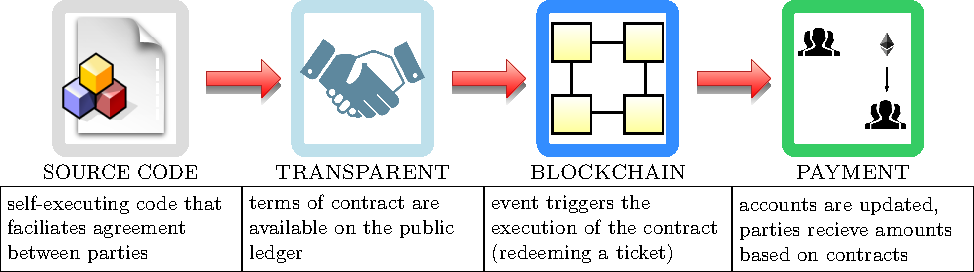
\includegraphics[width=1\linewidth]{smartContractsExp.pdf}
		\caption{Illustrating how a smart contract works}
		\label{fig:smartContracts}
	\end{figure}
\end{warpprint}

\begin{warpHTML}
	\begin{figure}[ht]
		\centering
		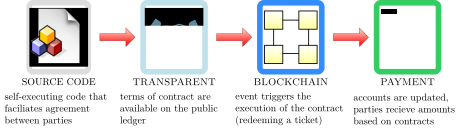
\includegraphics[width=1\linewidth]{smartContractsExp.svg}
		\caption{Illustrating how a smart contract works}
		\label{fig:smartContracts}
	\end{figure}
\end{warpHTML}

		In addition, irreversible and immutable transactions are a disadvantage that hackers can exploit. For example, an amateur coder killed the contract that allowed users to transfer Ether for the Parity \gls{Ethereum} Wallet, rendering 150 to 300 million dollars completely useless \cite{funnyJoke:Online}. Scrutinizing smart contracts and reducing bugs in production code is essential. The most common token standards, ERC20 and ERC721 interfaces outline how tokens work on Ethereum (See Appendix A).%An example of smart contract is available in Appendix A% \ref{lst:label}.
		
		% Rewrite here.
		The desirable properties of a \gls{blockchain} such as integrity and immutability of data, e.g., transactions and
		smart contracts, require an active mining pool. In a proof of work (POW) consensus  mechanism,  miners need to invest energy and resources,
		i.e. computational power, to participate in the consensus process and prevent tampering blocks. Additionally, miners are incentivized to run nodes that verify transactions. % through bitcoin or ether. %The investment must incentive miners to verify transactions and/or run nodes.%This investment has to be incentivized to prevent miners from not participating.
	
\subsection{Representation of Digital Assets on the Blockchain}

\paragraph{ERC20 Token Standard}

The ERC20 token standard allows any tokens on Ethereum to be re-used by other applications: from wallets to decentralized exchanges. This is the most commonly used token on the Ethereum network at the moment.

\paragraph{ERC721 Token Standard}

Non-fungible tokens are often used to represent scarality on the \gls{Ethereum} network.
The following standard (See Appendix A) allows for the implementation of a standard API for NFTs within smart contracts. This standard provides basic functionality to track and transfer NFTs.
NFTs can represent ownership over digital or physical assets. As seen in cryptozombies, this can also contain "dna".

\paragraph{Other Smart Contracts}
Other contracts in the Harvest system, such as the storefront contract allow creation of reward tokens (ERC721s), however, since deploying ERC721s is gas intensive, a separate reward deployer contract is instantiated and transfers ownership to the storefront. As shown in Figure \ref*{fig:gascost} better distributes the gas cost of deploying contracts. Additionally, the reward and storefront contract contain the ownable property (owned by the contract creator).

\begin{figure}[H]
\centering
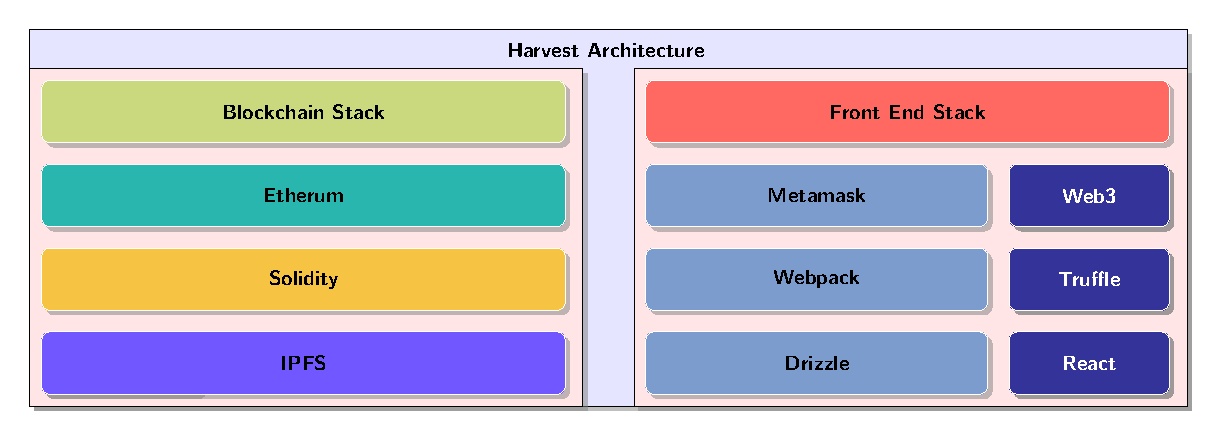
\includegraphics[width=1\linewidth]{Images/harvestArchitectureGood}
\caption{Architecture for smart contracts and front-end for harvest application}
\label{fig:harvestarchitecture}
\end{figure}

 Although determining the digital value of assets is challenging, the ability for a users to trade assets between themselves is essential for a decentralized marketplace. Implementation of a exchanger contract to buy/sell rewards and currencies are outside the scope of a proof of concept application.
%Participating music businesses will create a catalogue of valuable, real world offerings for the return of tokens from artists to the music business. Examples of products in this catalogue may include: studio recording sessions, record pressing, touring related costs, merchandise, and other goods and services. Music businesses will be encouraged to leverage existing business relationships to populate the catalogue of offerings. A music business offering this service may directly purchase rewards supply from vendors or work out rewards discounts that will be attractive to artists. 

%Music businesses who implement this tool will be differentiated from other distributors and rights managers. By adding an additional compensation and value to the way they compensate artists for plays, they will be able to create more loyalty and become even more attractive to potential artists. Every artist will benefit from the participation of previous artists as the economy of the MEC Rewards Program token grows. 


%	\end{minipage}
%%% New discussion
%%%%%%%%%%%%%%%%%%%%%%%%%%%%%%%%%%%%%%%%%%%%%%%%
%%%%%%% DISCUSSION %%%%%%%%%%%%%%%%%%%%%%%%%%%%%%
%%%%%%%%%%%%%%%%%%%%%%%%%%%%%%%%%%%%%%%%%%%%%%%%
\newpage
\section{Discussion}
 	The tools used in the harvest application are, a firefox/chrome plugin, metamask for connecting to the ethereum blockchain and testnets, the most popular framework for smart contract development truffle, and drizzle, which manages contract state.
		\subsection{Decentralized Applications}
		
		% Talk about drizzle metamask and truffle
		
		Decentralized systems are inherently more reliable, currently face scalability issues, and are trustless systems \cite{bitcoinWhitePaper:Online,ethereumWhitePaper:Online}. Fulfillment of smart contracts is limited due to off-chain information, logistical challenges in obtaining impartial or truthful inputs from stakeholders, and verification of transaction completion involving real-world assets. This suggests effectiveness of smart contracts is currently limited to digital assets rather than for physical assets.  In addition, translating legal-binding contracts to code is challenging because the majority of programmers lack a legal background.
		
		\begin{figure}[H]
		\centering
		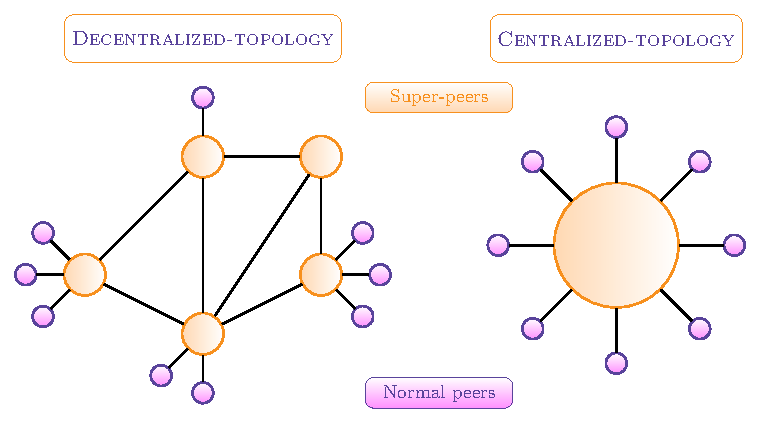
\includegraphics[width=0.7\linewidth]{DappVApp}
		\caption{Decentralized structure vs Centralized Structure}
		\label{fig:dappvapp}
		\end{figure}
		
		Despite shortcomings that involve transactional steps that are computational impossible to verify (package is delivered), performance of smart contracts is superior as transactions are tamper-proof.
		Additionally, reduction of ambiguity from usage of smart contracts is highly probable because only one interpretation is possible. Coding errors or bugs exist in every non-trivial application, therefore transactions through smart contracts intrinsically carry some risk. This implies protocols and prior real-world agreements are necessary to migrate risk when executing smart contracts. Furthermore, increased precision and detail for transactional inputs and outputs required for creating smart contracts would benefit all parties. 
		
% \subsection{Functionality of Harvest}

 % Talk about token trading, creating new ERC721s
 	
 \subsection{Trading digital currency for rewards}
 
 Artists will receive their tokens to a wallet where they can store and save or spend their tokens. Artists will be able to browse through the music business catalogue of goods and purchase items or services using their tokens. 
 
 What separates this project from a traditional rewards program (for example Airmiles or Aeroplan) would be the ability for artists (or any other token holder) to exchange tokens between each other easily using the Ethereum blockchain. Much of the work taking place in the music industry is conducted in exchange or in kind. The MEC Rewards Program could allow for artists to pass a value back and forth in exchange for tokens. The emergence of blockchain technology allows for these kinds of interactions to be transparent, trackable and scalable. 
 
 
 \begin{algorithm}[ht]
   \caption{Trading ERC20 tokens for ERC721 Rewards}\label{alg:tradingTokens}
   \hspace*{\algorithmicindent} \textbf{Input} uint256 \_ERC20Num, HarvestToken ERC20, RewardToken ERC721 \\
   \hspace*{\algorithmicindent} \textbf{Output} Number of ERC721 rewards returned
   \begin{algorithmic}[1]
     \Require
       \Statex More than one ERC721 must be traded.
       \Statex Transaction sender has \_ERC20Num number of ERC20 tokens.
       \Statex Make sure enough ERC721s are available (not owned by others).
       \Statex Permission to spend \_ERC20Num number of ERC20 tokens.
       %\Statex 
%     \Ensure
%       \Statex If I write \verb|\\| here, line's number will be wrong too.
     \Statex
     %\Comment{The number of distributed tokens is a global variable.}
     \State rate$ \gets ERC721.getRate()$ \Comment{gets rate of ERC20 to ERC721}
     \State  $ numOf721s \gets $ \_ERC20Num / rate
     \State ERC20.transferFrom(msg.sender,owner,\_ERC20Num) \Comment{owner is global variable}
     \State $ i \gets $ distributed\_token721 \Comment{Number of distributed 721 tokens is a global variable.}	
     \Repeat
	     \State ERC721.transferFrom(owner,msg.sender,i)
     \Until{$i>i+numOf721s$}
     \State distributed\_token721 = i
     
     \Return $numOf721s$
   
%     \If{$i = 1 \to n$} \Comment{This line's number should be 1}
%       \State ${\textit{HU}}_{i} \gets {\textit{NGU}}_{i} + {HU}_{i}$ \Comment{Comment}
%     \EndIf
   \end{algorithmic}
 \end{algorithm}
 
 Receiving rewards in Harvest requires an artist to approve the StoreFront contract to spend their ERC20 tokens with the expectation that a digital representation of a reward (ERC721) will be received. This requires the specific reward which could be recording time, or studio time to exist. In addition, only the owner of StoreFront can create new rewards and different kinds of rewards. Furthermore, in order for redemption to occur, real-world verification is necessary, then the result are recorded on the \gls{blockchain}. Since transactions cannot reversed adding thoughtful assert statements (reverse changes caused by ongoing transaction) is essential.
   
 % Creating new rewards in storefront 
 
 
   Assuming that ERC721 tokens will never be burned (destroyed), creating new tokens is simple. Since every ERC721 token has a unique id in its contract, incrementing the token id based on total supply of ERC721 is efficient.
  \begin{algorithm}[ht]
    \caption{Reward Creation Algorithm}\label{alg:algorithm2}
    \hspace*{\algorithmicindent} \textbf{Input}  RewardToken ERC721, uint256 numTokens \\
    \hspace*{\algorithmicindent} \textbf{Output} Returns true if new tokens are minted.
    
    \begin{algorithmic}[1]
      \Require
        \Statex Make sure the 721 reward token is registered (not counterfeit).
        \Statex Only the owner of a storefront can create rewards.

      \State $newTokenId=ERC721.totalSupply()$
      \Repeat
      	 \State ERC721.mint(address(this),i) \Comment{Reward are owned by storefront.}
      \Until{$i=newTokenId>i+numTokens$}
           \State distributed\_token721 = i
           
      \Return True
    \end{algorithmic}
  \end{algorithm}

\subsection{Rendering Rewards}

\subsubsection{Mapping unique info to components}



\begin{figure}[H]
\centering
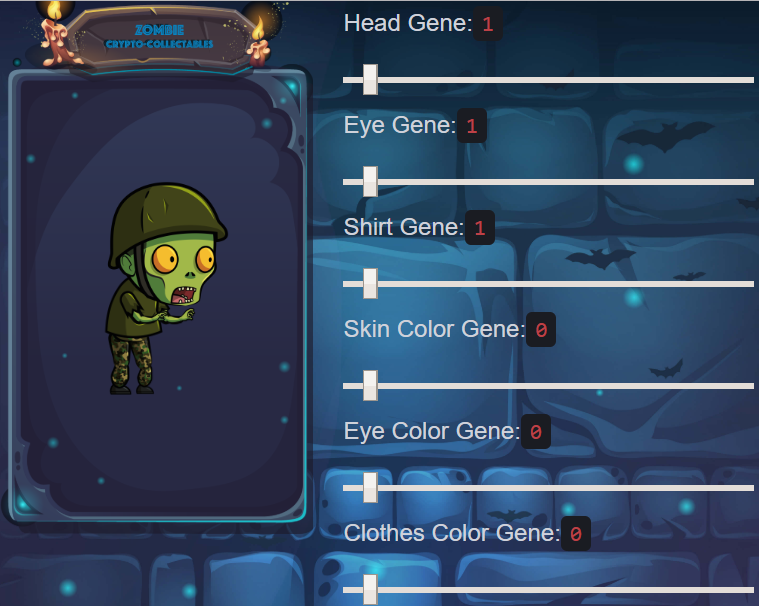
\includegraphics[width=0.7\linewidth]{cryptozombies}
\caption{Adjusting the appearance of the zombie by changing DNA values}
\label{fig:cryptozombies}
\end{figure}

Although ERC20 tokens are used as a to represent currency, representation of rewards can be done using ERC721. Since each ERC721 token has a unique token identifier, they can be displayed as digital collectables such as etheremon and cryptozombies \cite{cryptozombies} with their "dna" mapping to specific components.


As described in the popular solidity tutorial cryptozombies \cite{cryptozombies}, a zombie's appearance will be based on its "Zombie DNA". Zombie DNA is simple — it's a 16-digit integer, like:
% Break up into all parts for cryptzombies, if I am not lazy
\[
\underbrace{83}_{\text{head}} \qquad  \underbrace{56}_{\text{eyes}} \qquad \underbrace{281049284737}_{\text{Other parts}}
\]


Just like real DNA, different parts of this number will map to different traits. The first 2 digits map to the zombie's head type, the second 2 digits to the zombie's eyes, etc. One approach for rendering unique tokens in harvest, is to specific the type of reward which maps to an icon, and the colour values for the icon.

\[
\underbrace{83}_{\text{type}} \qquad  \underbrace{99}_{\text{red}} \qquad \underbrace{23}_{\text{blue}} \qquad \underbrace{13}_{\text{green}} \qquad 
\]

%\begin{figure}
%\centering

%\caption{Icons that could be used}
%\end{figure}
Despite simplicity of using predefined icons, distinguishing between different rewards is not guaranteed.
%\begin{figure}
%\centering
%
\includegraphics[width=0.7\linewidth]{blackIcons}
%\caption{Example Icons that represent rewards}
%\label{fig:blackicons}
%\end{figure}

\subsubsection{Using Decentralized Storage (IPFS)}


Allowing storefront owners to upload their own images that represents their reward is desirable. Decentralized storage such as IPFS is optional as the smart contract at minimum, could contain a link to the desired resource (image or text file), but having immutable, permanent links is beneficial. 
% cite eth-plot
 Large amounts of data can be addressed with IPFS, and the immutable, permanent IPFS links can be placed into a blockchain transaction. This timestamps and secures the content, without having to put the data on the chain itself.

Information to access the image (immutable and permanent IPFS links) is included inside a blockchain transaction. This secures the content without having to store the data on the chain which is quite expensive.   
 % Convert sequence diagram to state diagram showing how contracts are updated.
 % Include sequence diagram, or updated sequence diagram
%\begin{figure}
%\centering
%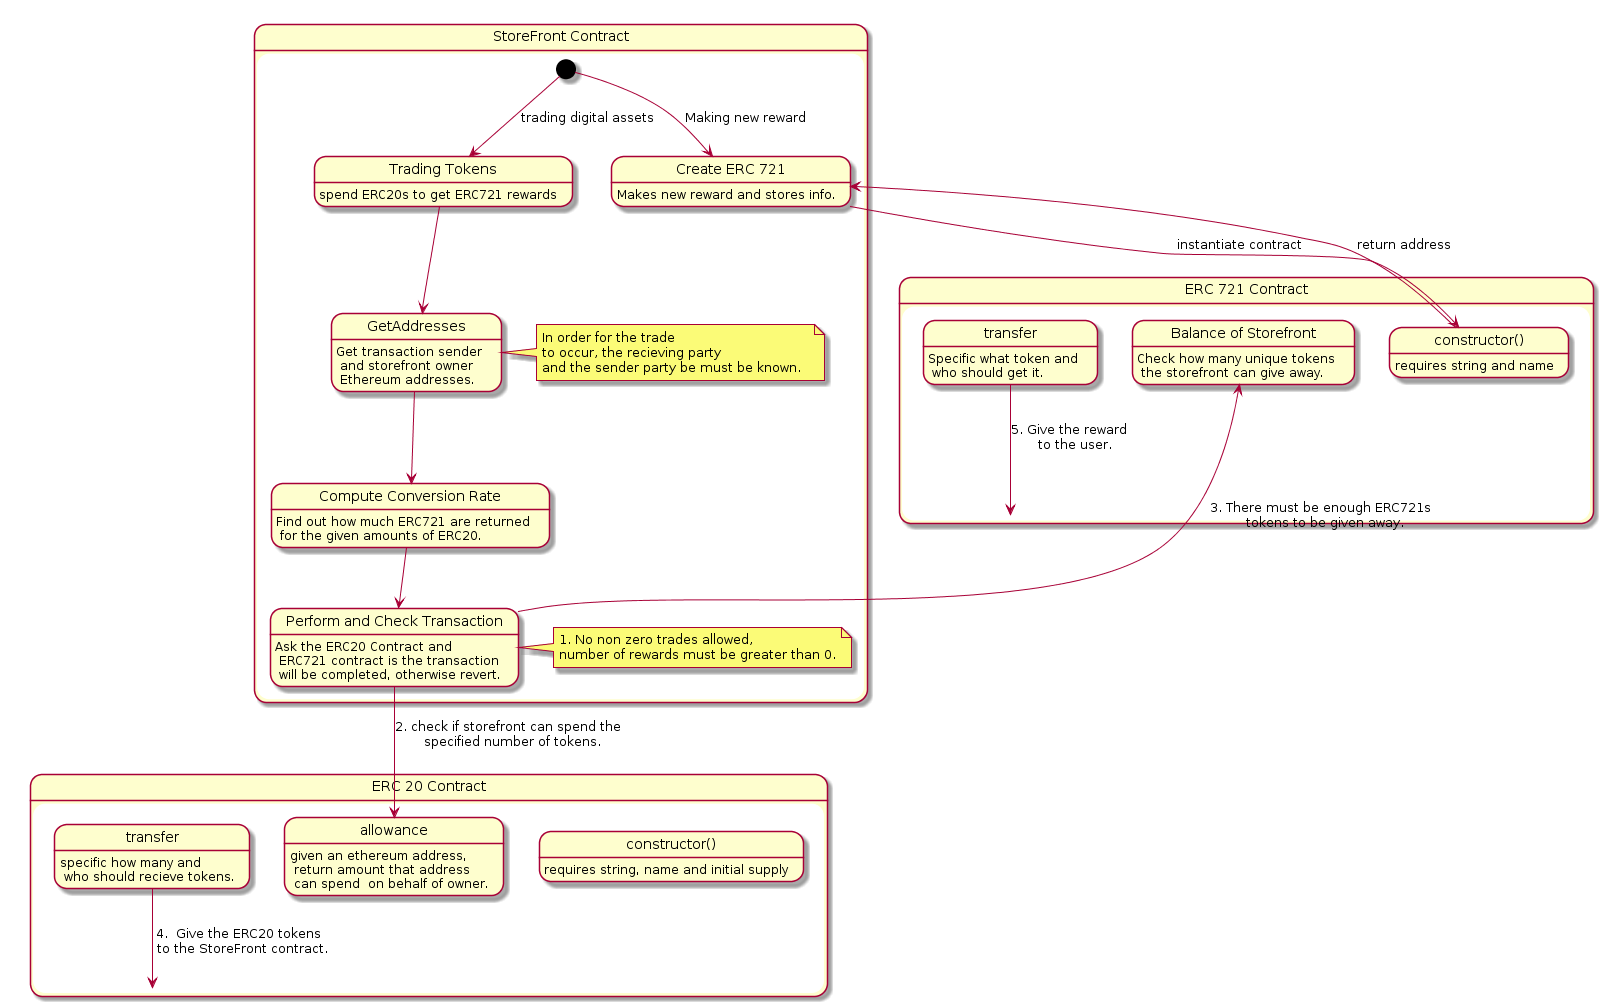
\includegraphics[width=1\linewidth]{StateDiagramENGR003}
%\caption{State Diagram when a User wants to trade tokens}
%\label{fig:statediagramengr003}
%\end{figure}
 \subsection{Optimization of smart contracts}
 
 On the \gls{Ethereum} network uses pay for transactions using \gls{gas}, this highly encourages programmers to create efficient \glspl{smart contract} that minimize costs to users while adhering to restrictive limitations for developing smart contracts. Performing calculations off-chain and verification in \glspl{smart contract} is highly desirable because writing to the blockchain is expensive. Balancing security, efficiency and simplicity is challenging, but extremely important as transactions cannot be reverted, and source code is publicly available. Currently, on Ethereum transactions sizes are limited to 32 kb, and \glspl{smart contract} cannot be larger than 24 kb.
 
 % Cite Ethereum Yellow paper
 %Efficiency in solidity 
  \begin{table}[H] 	\begin{tcolorbox}[tab2, tabularx={X||r|Y},title=Cost of Common Operations]
  		 Operation   &      Gas     &      Description \\\hline\hline
  		 ADD/SUB     &      3 &             Arithmetic  
  		  operation \\\hline
  		
  		 MUL/DIV      &     5 &            Arithmetic operation\\\hline
  		
  		 ADDMOD/MULMOD  &   8 &             Arithmetic operation \\ \hline 
  		  AND/OR/XOR     &   3    &  Bitwise logic operation \\ \hline 
  		  
  		   LT/GT/SLT/SGT/EQ & 3 &             Comparison operation \\ \hline
  		   
  		    POP       &        2        &     Stack operation \\ \hline 
  		     PUSH/DUP/SWAP  &    3 &             Stack operation \\ \hline 
  		      MLOAD/MSTORE  &    3     &        Memory operation\\ \hline 
  		     JUMP      &        8 &            Unconditional jump \\ \hline 
  		     JUMPI        &     10       &     Conditional jump \\ \hline
  		     SLOAD       &      200 &          Storage operation\\ \hline 
  		     SSTORE      &      5,000/20,000 &  Storage operation \\ \hline 
  		     BALANCE     &      400    &       Get balance of an account \\ \hline
  CREATE       &     32,000   &     Create a new account using CREATE
  		 \\\hline\hline
  
   CALL         &     25,000  &      Create a new account using CALL
  	\end{tcolorbox}
  	\caption{Cost of common operations in the Ethereum Virtual Machine }
  	\label{table:gas}
  \end{table}
  
  In addition, the gas limit for deploying smart contracts varies based on consensus with the miners, for example, on July 27, 2018, the gas limit for ropsten was 4.7 million units, but two days later on July 29, 2018 it reached 9.4 million units. Raising the gas limit is possible through increasing the amount of computation power available in the network, this may result because developers want to test large smart contracts. 
  % Dump etherscan blocks citation here\
  
  Oftentimes, in smart contract development, extending and customizing an existing contract (ERC20 and ERC721) is beneficial.
  Although some smart contracts may be deceitful small, inheritance and factory contract creation functionality can easily reach the gas limits set by the miners. 
  
  % Find citation again later
  
\begin{figure}[H]
\centering
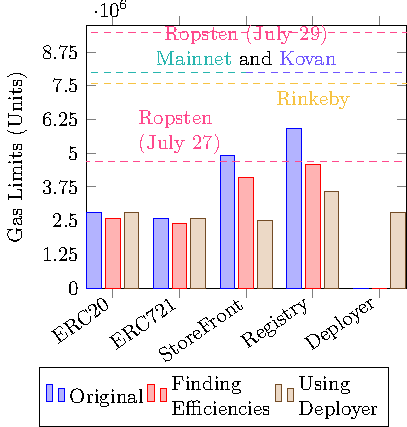
\includegraphics[width=1\linewidth]{Images/gasCost}
\caption{Optimization of Harvest Contracts and Gas Limits for Ethereum networks}
\label{fig:gascost}
\end{figure}
As shown in Figure \ref{fig:gascost} the original smart contracts were inefficient, reducing expensive operations (see Table \ref{table:gas}) such as storage and contract creation for factory contracts (deploying ERC721s) allows deployment on a testnet with for a relative low limit of 4.7 million units.

Previously, the Registry contract allowed creation and tracking of storefront contracts which in turn could create rewards, this resulted in a very costly Registry contract \ref{fig:gascost}.
In Solidity, creating smaller contracts with specific functionality is highly encouraged, for example having a reward deployer contract that only produces a new ERC721 contract and transfers ownership is highly efficient.
%Add Citation https://docs.google.com/spreadsheets/d/1n6mRqkBz3iWcOlRem_mO09GtSKEKrAsfO7Frgx18pNU/edit#gid=0
 


 
 
 
 
 

 \subsection{Limitations of Smart Contracts}
 % 24kb limit of data, 32 kb limit per transaction.
%	
\section{Discussion}
As shown in 
		Figure \ref{fig:DApp} \gls{DApp}, a user's transactions on the application is publicly broadcasting to the blockchain. 
		Implementing architecture for blockchain 
		applications 
		
		\footnote{Although, server blockchain architecture with an abstraction layer resemble traditional applications, other approaches are available such as offline signing with a public node, and client-blockchain in serverless apps and leveraging cloud infrastructure.} 
		
		adds an third layer to the standard client-server architecture 	\footnote{ \textbf{Signing Transactions}: One approach involves interacting with the JSON RPC interface of the \gls{Ethereum} node from the application to perform all blockchain operations.}.
		 Disadvantages of blockchain data storage include difficult retrieving relevant information (without an abstraction layer, the entire blockchain or a single transaction is returned), users will experience latency before transactions are validated, 	\footnote{For bitcoin, it takes 10 minutes before blocks of transactions are validated because of the mining process.}
		 
		  and writing to the blockchain is relatively expensive compared to traditional systems. Usage of interfaces such as the JSON RPC and/or cloud hosting 
	 solutions	
	 	 serve as a abstraction layer allowing databases to load publicly available data on the blockchain
	 	 % rewrite later 
	 	 for more efficient user interactions with that information. 

\begin{warpprint}
\begin{figure}[ht]
\begin{adjustbox}{center,max width=1.1\textwidth}
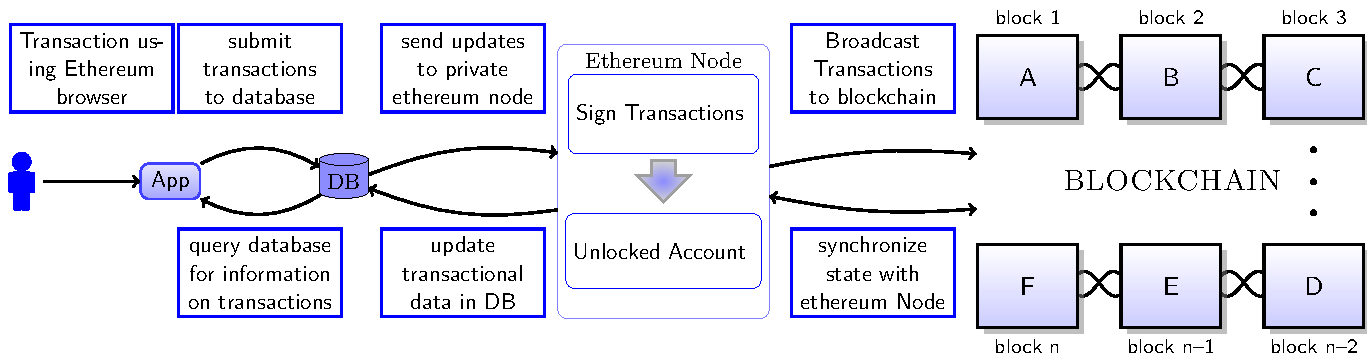
\includegraphics[width=1.2\linewidth]{Diagrams/blockchainInSimpleApp.pdf}
\end{adjustbox}
\caption{An example of server-blockchain architecture in a DAPP.}
\label{fig:DApp}
\end{figure}
\end{warpprint}

\begin{warpHTML}
\begin{figure}[ht]
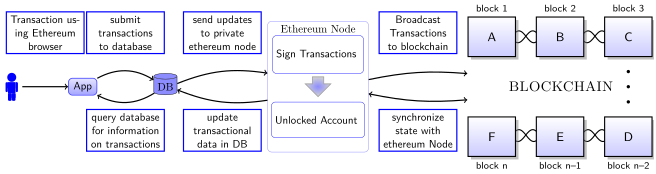
\includegraphics[width=1.2\linewidth]{Diagrams/blockchainInSimpleApp.svg}
\caption{An example of server-blockchain architecture in a DAPP.}
\label{fig:DApp}
\end{figure}
\end{warpHTML}

\begin{warpprint}
\begin{table}[]
\centering
\caption{Sample Decision Matrix for designing a blockchain system}
\arrayrulecolor{white}
\arrayrulewidth=1pt
\renewcommand{\arraystretch}{1.5}
\rowcolors[\hline]{3}{.!50!white}{}
\begin{tabular}{D E A B C }
\multicolumn{1}{l}{}      & \multicolumn{1}{c}{Existing Systems}    & \multicolumn{3}{c}{BlockChain Systems}                                                                                    \\
\multicolumn{1}{c}{Criteria}                 & \multicolumn{1}{c}{Centralized} & \multicolumn{1}{c}{Public} & \multicolumn{1}{c}{Permissioned} & \multicolumn{1}{c}{Private} \\
speed and latency         &                                         &                                       &                                             &                                        \\
scale and volume          &                                         &                                       &                                             &                                        \\
security and immutablity  &                                         &                                       &                                             &                                        \\
storage capacity          &                                         &                                       &                                             &                                        \\
transparency              &                                         &                                       &                                             &                                        \\
\multicolumn{1}{c}{Total} &                                         &                                       &                                             &                                       
\end{tabular}
\end{table}
\end{warpprint}

% HTML VERSION OF TABLE
\begin{warpHTML}

A generic message here? 

\begin{table}
\centering
\caption{My caption}
\begin{tabular}{cllll}
\multicolumn{1}{l}{}      & \multicolumn{1}{c}{Current Solution}    & \multicolumn{3}{c}{Alternative Solutions}                                                                                    \\
Criteria                  & \multicolumn{1}{c}{Centralized Systems} & \multicolumn{1}{c}{Public Blockchain} & \multicolumn{1}{c}{Permissioned Blockchain} & \multicolumn{1}{c}{Private Blockchain} \\
speed and latency         &                                         &                                       &                                             &                                        \\
scale and volume          &                                         &                                       &                                             &                                        \\
security and immutablity  &                                         &                                       &                                             &                                        \\
storage capacity          &                                         &                                       &                                             &                                        \\
transparency              &                                         &                                       &                                             &                                        \\
\multicolumn{1}{l}{Total} &                                         &                                       &                                             &                                       
\end{tabular}
\end{table}
\end{warpHTML}
Continued research into \gls{blockchain} technologies is necessary as innovations mitigate scalability issues, widespread adoption of cryptocurrency and technologies evolutions address the shortcomings of blockchain. In trustless systems tampering or modification of transactional history is extremely difficult. This suggests that smart contracts can greatly improve transactions, however, issues including scalability, reversing fraudulent activity and reduction of contract deployment hinder mass adoption.

All computer programs have bugs, by limiting complexity of smart contracts,  using reliable standards highly audited packages, and using software security analyze tools risk can be greatly reduced. 
\begin{figure}[H]
\centering
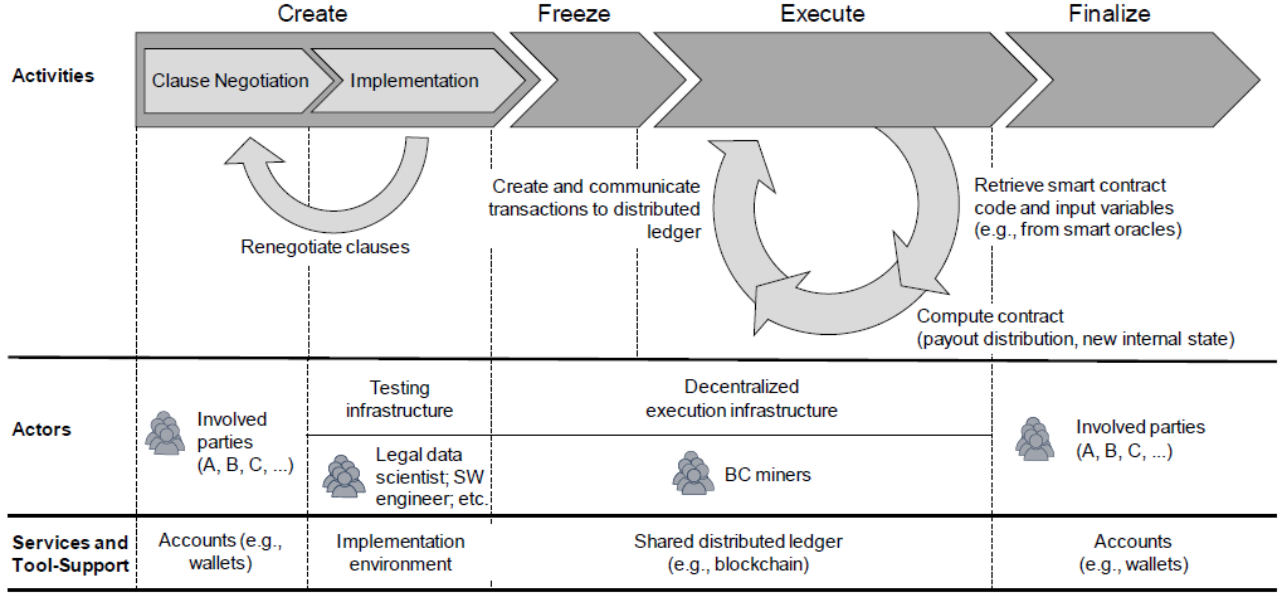
\includegraphics[width=1\linewidth]{smartContractCreation}
\caption{Lifecycle of Smart Contract Creation \cite{Sillaber2017}}
\label{fig:smartcontractcreation}
\end{figure}

As shown in figure \ref{fig:smartcontractcreation} multiple parties are required to create comprehensive smart contract, input from legal professions and negotiations are required. Additionally, unlikely other forms of software, iterative releases of \glspl{smart contract} is inefficient.
% Talk about the variable limits and how they are somtimes raised for smart contract testing.

% https://ropsten.etherscan.io/block/3734489

% https://ropsten.etherscan.io/block/3721380

\newpage 
%\section{Conclusion}
Adopting JIRA has benefited ME by reducing response time, improving record keeping and sharpening communication. Although JIRA has benefited the organization by improving efficiency, lack of education resulting in underutilisation of dashboards and filters, occasional performance issues causing issue backlogs to pile up, and perceived unreliability for sending emails.  Agile software development methodologies such as Scrum and Kanban are supported by the JIRA suite of applications. JIRA has add-ons that extend functionality will complexity ranging from a single feature to full product.  Interestingly, when JIRA is integrated with Confluence usage of both applications will increase because jumping between application is quick and simple. \\

In order to streamline the adoption of \gls{Confluence}, usage intentions must be conveyed as well as detailed guidance on how to use it. Confluence is wiki software used to create knowledge bases, centralize information into a single system and for technical documentation. Useful features of Confluence include integration with \gls{JIRA}, word processing, and team collaboration.  Connecting JIRA and Confluence applications allows enable users to rapidly switch between applications.  Overall, JIRA and Confluence are software tools that improve productivity and organization within BTI IM.
\section{Conclusion}
	

	
   Blockchain technology is disrupting many industries. The economy of the music industry has yet to recover from the last disruption, the proliferation of digital music first through mp3s and now streaming platforms. The Ethereum network provides key standards such as ERC20 and ERC721 to represent digital currency and scarcity in the blockchain. Understanding ownership and nuances of Solidity is key to creation of bug-free and efficient smart contracts. As shown in Figure \ref{fig:gascost} shifting specific functionality such as factory contracts is essential to meeting the gas limits.
   
   
   Artists may receive compensation based on total listens from streaming services, but there are many stories which outline how little profit artists actually receive from these royalties. This is an issue even for massively successful artists, let alone emerging or independent artists. The MEC Rewards Program aims to use new technology (the blockchain and decentralized apps) to bring transparency and innovation to the compensation of artists in the new digital economy, while creating a valuable business proposition for industry. Representation of digital rewards could involve storing an image online and including that url inside of a smart contract. Overall, blockchain is an effective platform for a decentralized marketplace.
\newpage
% \section{Recommendations}
 
 
  
Obviously continued researching into \gls{blockchain} technologies is necessary as innovations such as permissioned blockchains such as \gls{HyperLedger Composer} and \gls{side chains} continue to address some shortcomings of blockchain. In trustless systems tampering or modification of transactional history is extremely difficult. This suggests that smart contracts can greatly improve transactions, however, issues including scalability, reversing fraudulent activity and reduction of contract deployment hinder mass adoption.

All computer programs have bugs, by limiting complexity of smart contracts,  using reliable standards highly audited packages, and using software security analyze tools risk can be greatly reduced. Continuing to monitor technology innovations such ever-increasing computational power is important to ensure cracking private keys remain uneconomical see Figure \ref{security:fig2}.

Provided a deterministic set of inputs and outputs, with computational verifiable conditions, using smart contracts is beneficial.
Increasing awareness about \gls{blockchain} technologies, so that the average person understands the limitations of smart contracts and in what situations they can be useful.

\newpage
\section{Recommendations}
	
	Additionally, storage and contract creation is expensive, so optimization of smart contracts is essential. Furthermore, usage of \glspl{smart contract} completely automated transactions are limited to computational verifiable events, otherwise users could falsify input data. As adoption of blockchain technology grows, and scalability of the Ethereum network increases, decentralized applications will become a viable alternative.
	
	
	Artists will receive their tokens to a wallet where they can store and save or spend their tokens. Artists will be able to browse through the music business’ catalogue of goods and 'purchase' items or services using their tokens. By adding an additional compensation and value to the way they compensate artists for plays, they will be able to create more loyalty and become even more attractive to potential artists.
	
	Provided a deterministic set of inputs and outputs, with computational verifiable conditions, using smart contracts is beneficial. Increasing awareness about \gls{blockchain} technologies, so that the average person understands the limitations of smart contracts and suitable applications is a key aspect in increasing adoption and widespread acceptance of \gls{blockchain} technologies.
	
	
%%%%%%%%%%%%%%%%%%%%%%%%%%%%%%%%%%%%%%%%%%%%%%
%%%% END Main Content %%%%%%%%%%%%%%%%%%%
%%%%%%%%%%%%%%%%%%%%%%%%%%%%%%%%%%%%%%%%%%%%%%

%%%%%%%%%%%%%%%%%%%%%%%%%%%%%%%%%%%%%%%%%%%%%%
%%% BACK MATTER, printing References %%%%%%%%%
%%%%%%%%%%%%%%%%%%%%%%%%%%%%%%%%%%%%%%%%%%%%%%
\renewcommand\bibname{References} % Change bibliography to references

% nocite prints all references even if they were not used
% \nocite{*}
\newpage 
 \printbibliography
 
\linespread{1}

\newpage 
\begin{appendices}
\section{Token Standards}
%\lstinputlisting[
%language   = C,
%basicstyle = \ttfamily,
%style		= default,
%%frame      = single,
%caption    = {Caesar Cipher for CSC 111},]
%{Code/cipher.c}
\begin{lstlisting}[language=Solidity,caption=ERC20 Token Standard Interface]
pragma solidity ^0.4.20;
contract ERC20Interface {
    function totalSupply() public constant returns (uint);
    function balanceOf(address tokenOwner) public constant returns (uint balance);
    function allowance(address tokenOwner, address spender) public constant returns (uint remaining);
    function transfer(address to, uint tokens) public returns (bool success);
    function approve(address spender, uint tokens) public returns (bool success);
    function transferFrom(address from, address to, uint tokens) public returns (bool success);

    event Transfer(address indexed from, address indexed to, uint tokens);
    event Approval(address indexed tokenOwner, address indexed spender, uint tokens);
}
\end{lstlisting}

\begin{lstlisting}[language=Solidity, caption=ERC721 Token Standard Interface]
pragma solidity ^0.4.20;

contract ERC721 {
    event Transfer(address indexed _from, address indexed _to, uint256 indexed _tokenId);
    event Approval(address indexed _owner, address indexed _approved, uint256 indexed _tokenId);
    event ApprovalForAll(address indexed _owner, address indexed _operator, bool _approved);
    function balanceOf(address _owner) external view returns (uint256);
    function ownerOf(uint256 _tokenId) external view returns (address);
    function safeTransferFrom(address _from, address _to, uint256 _tokenId, bytes data) external payable;
    function safeTransferFrom(address _from, address _to, uint256 _tokenId) external payable;
    function transferFrom(address _from, address _to, uint256 _tokenId) external payable;
    function approve(address _approved, uint256 _tokenId) external payable;
    function setApprovalForAll(address _operator, bool _approved) external;
    function getApproved(uint256 _tokenId) external view returns (address);
    function isApprovedForAll(address _owner, address _operator) external view returns (bool);
}

\end{lstlisting}
\end{appendices}
\end{document}

%%%%%%%%%%%%%%%%
COMMON COMMANDS:
%%%%%%%%%%%%%%%%
% IMAGES
\begin{figure}[H]
	\begin{center}
		\includegraphics[width=0.6\textwidth]{RTL_SCHEM.png}
	\end{center}
	\caption{A screenshot of the RTL Schematics produced from the Verilog code.}
	\label{RTL}
\end{figure}

% SUBFIGURES IMAGES
\begin{figure}[H]
	\centering
	\subfloat[LED4 Period]{\label{fig:Per4}\includegraphics[width=0.4\textwidth]{period_led4.png}} \\                
	\subfloat[LED5 Period]{\label{fig:Per5}\includegraphics[width=0.4\textwidth]{period_led5.png}}
	\subfloat[LED6 Period]{\label{fig:Per6}\includegraphics[width=0.4\textwidth]{period_led6.png}}
	\caption{Period of LED blink rate captured by osciliscope.}
	\label{fig:oscil}
\end{figure}

% CITATIONS
\cite{CitationName}

% GLOSSARY ENTRY
\newglossaryentry{api}
{
	name={API},
	description={An Application Programming Interface (API) is a particular set
		of rules and specifications that a software program can follow to access and make use of the services and resources provided by another particular software program that implements that API},
	first={Application Programming Interface (API)},
	long={Application Programming Interface}
}
% INSERT SOURCE CODE
\lstinputlisting[
language=SQL,
basicstyle = \ttfamily,
style=			Oracle,
%frame      = single,
caption    = {Sample SQL Query},]
{Code/Data.sql}

% FANCY TABLE
\begin{table}
	\begin{center}
	\begin{tabular}{@{} l *4c @{}}
		\toprule
		\multicolumn{1}{c}{Models}    & A  & B  & C  & D  \\ 
		\midrule
		Model $X$ & X1 & X2 & X3 & X4 \\ 
		Model $Y$ & Y1 & Y2 & Y3 & Y4 \\
		\bottomrule
	\end{tabular}
	\caption{Caption}
	\end{center}
\end{table}

% TEXT TABLE
\begin{table}
	\begin{center}
		\begin{tabular}{|l|c|c|l|}
			x & x & x & x \\ \hline
			x & x & x & x \\
			x & x & x & x \\ \hline
		\end{tabular}
		\caption{Caption}
		\label{label}
	\end{center}
\end{table}

% MATHMATICAL ENVIRONMENT
$ 8 = 2 \times 4 $

% CENTERED FORMULA
\[  \]

% NUMBERED EQUATION
\begin{equation}

\end{equation}

% ARRAY OF EQUATIONS (The splat supresses the numbering)
\begin{align*}

\end{align*}

% NUMBERED ARRAY OF EQUATIONS
\begin{align}

\end{align}

% ACCENTS
\dot{x} % dot
\ddot{x} % double dot
\bar{x} % bar
\tilde{x} % tilde
\vec{x} % vector
\hat{x} % hat
\acute{x} % acute
\grave{x} % grave
\breve{x} % breve
\check{x} % dot (cowboy hat)

% FONTS
\mathrm{text} % roman
\mathsf{text} % sans serif
\mathtt{text} % Typewriter
\mathbb{text} % Blackboard bold
\mathcal{text} % Caligraphy
\mathfrak{text} % Fraktur

\textbf{text} % bold
\textit{text} % italic
\textsl{text} % slanted
\textsc{text} % small caps
\texttt{text} % typewriter
\underline{text} % underline
\emph{text} % emphasized

\begin{tiny}text\end{tiny} % Tiny
\begin{scriptsize}text\end{scriptsize} % Script Size
\begin{footnotesize}text\end{footnotesize} % Footnote Size
\begin{small}text\end{small} % Small
\begin{normalsize}text\end{normalsize} % Normal Size
\begin{large}text\end{large} % Large
\begin{Large}text\end{Large} % Larger
\begin{LARGE}text\end{LARGE} % Very Large
\begin{huge}text\end{huge}   % Huge
\begin{Huge}text\end{Huge}   % Very Huge

%   \Gls{agile} software development uses repeatable brief cycles called 
%   \glspl{sprint} that focus on short-term deliverables.
\begin{figure}
	\caption{A picture323}
\end{figure}
\begin{table}[H]
	\begin{center}
		\begin{tabular}{cccc}
			\toprule 
			Nucleus & \textit{I} & Natural Abundance / \% & Larmor Frequency @ 7T \\
			\midrule
			\rowcolor{black!20} \textsuperscript{1}H & \sfrac{1}{2} & 99.98 & 298.0 \\
			\textsuperscript{2}H & 1 & 0.02 & 45.7 \\
			\rowcolor{black!20} \textsuperscript{12}C & 0 & 98.90 & - \\
			\textsuperscript{13}C & \sfrac{1}{2} & 1.10 & 74.9 \\
			\rowcolor{black!20} \textsuperscript{14}N & 1 & 99.60 & 21.5 \\
			\textsuperscript{15}N & \sfrac{1}{2} & 0.40 & 30.2 \\
			\rowcolor{black!20} \textsuperscript{16}O & 0 & 99.96 & - \\
			\textsuperscript{17}O & \sfrac{1}{2} & 0.04 & 40.4 \\
			\bottomrule
		\end{tabular}
		\caption{Numbers232323}
	\end{center}
\end{table}

%%% COMPLETE TABLE EXAMPLE %%%%
\newcommand{\head}[1]{\textnormal{\textbf{#1}}}
\newcommand{\normal}[1]{\multicolumn{1}{l}{#1}}
\begin{table}
	\centering
	\begin{tabular}{@{}l*2{>{\textbackslash\ttfamily}l}%
			l<{Example text}l@{}}
		\toprule[1.5pt]
		& \multicolumn{2}{c}{\head{Input}}
		& \multicolumn{2}{c}{\head{Output}}\\
		& \normal{\head{Command}} & \normal{\head{Declaration}}
		& \normal{\head{Single use}} & \head{Combined}\\
		\cmidrule(lr){2-3}\cmidrule(l){4-5}
		\multirow{3}{*}{Family} &  textrm & rmfamily & \rmfamily & \\
		& textsf & sffamily & \sffamily & \\
		& texttt & ttfamily & \ttfamily & \\
		\cmidrule(lr){2-3}\cmidrule(lr){4-4}
		\multirow{2}{1.1cm}{Weight} & textbf & bfseries & \bfseries
		& \multirow{2}{1.8cm}{\sffamily\bfseries Bold and sans-serif} \\
		& textmd & mdseries & \mdseries & \\
		\cmidrule(lr){2-3}\cmidrule(lr){4-4}
		\multirow{4}{*}{Shape} & textit & itshape & \itshape & \\
		& textsl & slshape & \slshape &
		\multirow{2}{1.8cm}{\sffamily\slshape Slanted and sans-serif}\\
		& textsc & scshape & \scshape & \\
		& textup & upshape & \upshape & \\
		\cmidrule(lr){2-3}\cmidrule(lr){4-4}
		Default & textnormal & normalfont & \normalfont & \\
		\bottomrule[1.5pt]
	\end{tabular}
	\caption{\LaTeX\ font selection}
\end{table}
%%%%    END TABLE EXAMPLE   %%%%%

%%%% TABLE EXAMPLE %%%%
\newcolumntype{Y}{>{\raggedleft\arraybackslash}X}

\tcbset{tab1/.style={fonttitle=\bfseries\large,fontupper=\normalsize\sffamily,
		colback=yellow!10!white,colframe=red!75!black,colbacktitle=orange!40!white,
		coltitle=black,center title,freelance,frame code={
			\foreach \n in {north east,north west,south east,south west}
			{\path [fill=red!75!black] (interior.\n) circle (3mm); };},}}

\tcbset{tab2/.style={enhanced,fonttitle=\bfseries,fontupper=\normalsize\sffamily,
		colback=yellow!10!white,colframe=red!50!black,colbacktitle=yellow!40!white,
		coltitle=black,center title}}
\begin{table}
	\begin{tcolorbox}[tabularx={X||Y|Y|Y|Y||Y},title=My table]
		Group & One & Two & Three & Four & Sum\\\hline\hline
		Red & 1000.00 & 2000.00 & 3000.00 & 4000.00 & 10000.00\\\hline
		Green & 2000.00 & 3000.00 & 4000.00 & 5000.00 & 14000.00\\\hline
		Blue & 3000.00 & 4000.00 & 5000.00 & 6000.00 & 18000.00\\\hline\hline
		Sum & 6000.00 & 9000.00 & 12000.00 & 15000.00 & 42000.00
	\end{tcolorbox}
	\caption{Another Great Table}
\end{table}
\begin{table}
	\begin{tcolorbox}[tab1, tabularx={X||Y|Y|Y|Y||Y}]
		Group & One & Two & Three & Four & Sum\\\hline\hline
		Red & 1000.00 & 2000.00 & 3000.00 & 4000.00 & 10000.00\\\hline
		Green & 2000.00 & 3000.00 & 4000.00 & 5000.00 & 14000.00\\\hline
		Blue & 3000.00 & 4000.00 & 5000.00 & 6000.00 & 18000.00\\\hline\hline
		Sum & 6000.00 & 9000.00 & 12000.00 & 15000.00 & 42000.00
	\end{tcolorbox}
	\caption{Great Table}
\end{table}
\begin{table}
	\begin{tcolorbox}[tab2, tabularx={X||Y|Y|Y|Y||Y},title=My table]
		Group & One & Two & Three & Four & Sum\\\hline\hline
		Red & 1000.00 & 2000.00 & 3000.00 & 4000.00 & 10000.00\\\hline
		Green & 2000.00 & 3000.00 & 4000.00 & 5000.00 & 14000.00\\\hline
		Blue & 3000.00 & 4000.00 & 5000.00 & 6000.00 & 18000.00\\\hline\hline
		Sum & 6000.00 & 9000.00 & 12000.00 & 15000.00 & 42000.00
	\end{tcolorbox}
	\caption{Good Table}
\end{table}
%%%% END TABLE EXAMPLE %%%%

%ANOTHER TABLE EXAMPLE
\setlist{nolistsep}
\definecolor{green}{HTML}{66FF66}
\definecolor{myGreen}{HTML}{009900}

%\renewcommand{\familydefault}{\sfdefault}


\begin{table}
	\begin{center}
		\begin{tabularx}{\textwidth}[t]{XX}
			\arrayrulecolor{green}\hline
			\textbf{\textcolor{myGreen}{Goal 1 Eradicate Extreme Poverty}} & \\
			\hline
			Target 1.A Halve, between 1990 and 2015, the proportion of the people whose income is less than \$1 a day. & 
			\begin{minipage}[t]{\linewidth}%
				\begin{itemize}
					\item[1.1] Proportion of population below \$1 purchasing power parity (PPP) a day$^a$
					\item[1.2] Poverty Gap ratio [incidence x depth of poverty]
					\item[1.3] Share of the poorest quintile in national consumption
				\end{itemize} 
			\end{minipage}\\
			
			\arrayrulecolor{black}\hline
			
			Target 1.B Achieve full and productive employment and decent work for all, including women and young people &
			\begin{minipage}[t]{\linewidth}%
				\begin{itemize}
					\item[1.4] Growth of GDP per person employed 
					\item[1.5] Employment to population ratio
					\item[1.6] Proportion of employed people living below \$1 (PP) a day
					\item[1.7] Proportion of own-account and contribution family workers in total employment
				\end{itemize} 
			\end{minipage}\\
			
			\hline
			
			Target 1.C Halve, between 1990 and 2015, the proportion of people who suffer from hunger &
			\begin{minipage}[t]{\linewidth}%
				\begin{itemize}
					\item[1.8] Prevalence of underweight children under five years of age
					\item[1.9] Proportion of population below minimum level of dietary energy consumption
				\end{itemize}
			\end{minipage}\\
			
			\arrayrulecolor{green}\hline
			\textbf{\textcolor{myGreen}{Goal 2 Achieve universal primary education}} \\
			\hline
			
			Target 2.A Ensure that by 2015 children everywhere, boy and girls alike, will be able to complete a full course of primary schooling. &
			\begin{minipage}[t]{\linewidth}%
				\begin{itemize}
					\item[2.1] Net enrollment ratio in primary education
					\item[2.2] Proportion of pupils starting grade 1 who reach last grade of primary education
					\item[2.3] Literacy rate of 15- to 24-year-olds, women and men
				\end{itemize}
			\end{minipage}\\
			
			\hline
			\multicolumn{2}{l}{%
				\textbf{\textcolor{myGreen}{Goal 3 Promote gender equality and empower women}}} \\
			\hline
			
			Target 3.A Eliminate gender disparity in primary and secondary education, preferably by 2005, and in all levels of education no later than 2015 &
			\begin{minipage}[t]{\linewidth}%
				\begin{itemize}
					\item[3.1] Ratios of girls to boys in primary, secondary and tertiary education
					\item[3.2] Share of women in wage employment in the non-agricultural sector.
				\end{itemize} 
			\end{minipage}
		\end{tabularx}
	\end{center}
	\caption{Great table to use}
\end{table}
% END ANOTHER TABLE EXAMPLE
\begin{figure}
	\caption{Another picture2323}
\end{figure}


\lstinputlisting[
language=SQL,
basicstyle = \ttfamily,
style=			Oracle,
caption    = {Sample SQL Query},]
{Code/Data.sql}	

\begin{table}
	\begin{center}
		\begin{tabular}{ |l|l|l| }
			\hline
			\multicolumn{3}{ |c| }{Team sheet} \\
			\hline
			Goalkeeper & GK & Paul Robinson \\ \hline
			\multirow{4}{*}{Defenders} & LB & Lucas Radebe \\
			& DC & Michael Duburry \\
			& DC & Dominic Matteo \\
			& RB & Didier Domi \\ \hline
			\multirow{3}{*}{Midfielders} & MC & David Batty \\
			& MC & Eirik Bakke \\
			& MC & Jody Morris \\ \hline
			Forward & FW & Jamie McMaster \\ \hline
			\multirow{2}{*}{Strikers} & ST & Alan Smith \\
			& ST & Mark Viduka \\
			\hline
		\end{tabular}
	\end{center}
	\caption{Table Title}
\end{table}

\begin{table} 
	\begin{center}
		\begin{tabular}{cccccccc} \toprule
			{$m$} & {$\Re\{\underline{\mathfrak{X}}(m)\}$} & {$-\Im\{\underline{\mathfrak{X}}(m)\}$} & {$\mathfrak{X}(m)$} & {$\frac{\mathfrak{X}(m)}{23}$} & {$A_m$} & {$\varphi(m)\ /\ ^{\circ}$} & {$\varphi_m\ /\ ^{\circ}$} \\ \midrule
			1  & 16.128 & +8.872 & 16.128 & 1.402 & 1.373 & -146.6 & -137.6 \\
			2  & 3.442  & -2.509 & 3.442  & 0.299 & 0.343 & 133.2  & 152.4  \\
			3  & 1.826  & -0.363 & 1.826  & 0.159 & 0.119 & 168.5  & -161.1 \\
			4  & 0.993  & -0.429 & 0.993  & 0.086 & 0.08  & 25.6   & 90     \\ \midrule
			5  & 1.29   & +0.099 & 1.29   & 0.112 & 0.097 & -175.6 & -114.7 \\
			6  & 0.483  & -0.183 & 0.483  & 0.042 & 0.063 & 22.3   & 122.5  \\
			7  & 0.766  & -0.475 & 0.766  & 0.067 & 0.039 & 141.6  & -122   \\
			8  & 0.624  & +0.365 & 0.624  & 0.054 & 0.04  & -35.7  & 90     \\ \midrule
			9  & 0.641  & -0.466 & 0.641  & 0.056 & 0.045 & 133.3  & -106.3 \\
			10 & 0.45   & +0.421 & 0.45   & 0.039 & 0.034 & -69.4  & 110.9  \\
			11 & 0.598  & -0.597 & 0.598  & 0.052 & 0.025 & 92.3   & -109.3 \\ \bottomrule
		\end{tabular}
	\end{center}
	\caption{Table Title}
\end{table}


Use one of the nice tables.


% See https://docs.google.com/spreadsheets/d/1n6mRqkBz3iWcOlRem_mO09GtSKEKrAsfO7Frgx18pNU/edit#gid=0

% See https://cryptozombies.io/en/lesson/1/chapter/1